\documentclass[11pt,a4paper]{article}

% Definition des marges du document
\setlength{\topmargin}{0cm}
\setlength{\headheight}{0.4cm}
\setlength{\headsep}{0.8cm}
\setlength{\footskip}{1cm}
\setlength{\textwidth}{17cm}
\setlength{\textheight}{25cm}
\setlength{\voffset}{-1.5cm}
\setlength{\hoffset}{-0.5cm}
\setlength{\oddsidemargin}{0cm}
\setlength{\evensidemargin}{0cm}

% Inclusion des packages
\usepackage{graphicx} % inclusion des figures
\usepackage{subfig}
\usepackage{amsmath} % collection de symboles mathématiques
\usepackage{amssymb} % collection de symboles mathématiques
\usepackage{amsthm,ifsym}
\usepackage[utf8]{inputenc}       % utilisation directe des caractères accentués sur pc
\usepackage[T1]{fontenc} % codage moderne des caractères sous Latex
\usepackage[french]{babel}           % style français
\usepackage{listings}
\usepackage{tabularx} % gestion avancée des tableaux
\usepackage{psfrag} % remplacement du texte d'une figure ps par du texte latex
\usepackage{sistyle} % mise en forme des unités
\usepackage{epstopdf}
\usepackage{eurosym} % symbole €

\def\€{\euro{}}

\usepackage{color} % gestion de différentes couleurs

\definecolor{linkcolor}{rgb}{0,0,0.6} % définition de la couleur des liens pdf
\usepackage[ pdftex,colorlinks=true,
pdfstartview=FitV,
linkcolor= linkcolor,
citecolor= linkcolor,
urlcolor= linkcolor,
hyperindex=true,
hyperfigures=false]
{hyperref} % fichiers pdf 'intelligents', avec des liens entre les références, etc.

\usepackage{fancyhdr} % entêtes et pieds de pages personnalisés

\newtheorem{theorem}{Théorème}[section]
\newtheorem{proposition}[theorem]{Proposition}
\newtheorem{lemma}[theorem]{Lemma}
\newtheorem{corollary}[theorem]{Corollary}
\newtheorem{definition}[theorem]{Definition}
\newtheorem{remark}[theorem]{Remark}

% définition de l'entête et du pied de page
\pagestyle{fancy}
\fancyhead[L]{\scriptsize \textsc{Méthode des volumes finis pour la dynamique des fluides relativistes}}
\fancyhead[R]{\scriptsize \textsc{Marvin Lasserre}}
\fancyfoot[C]{ \thepage}

% commande d'annulation du correcteur typographique du package [francais]{babel} qui force l'espace avant ':' (parfois utile pour la bibliographie)
\makeatletter
\@ifpackageloaded{babel}%
        {\newcommand{\nospace}[1]{{\NoAutoSpaceBeforeFDP{}#1}}}%  % !! double {{}} pour cantonner l'effet à l'argument #1 !!
        {\newcommand{\nospace}[1]{#1}}
\makeatother

% commande de déplacement d'un objet
\newcommand{\drawat}[3]{\makebox[0pt][l]{\raisebox{#2}{\hspace*{#1}#3}}}

\begin{document}

% Pour faciliter la mise en forme de la page du titre, on supprime l'indentation automatique en début de paragraphe
\setlength{\parindent}{0pt}

% Pas d'en-tête ni de pied pour la première page
\thispagestyle{empty}


\includegraphics[height=2cm]{logos/logoens.eps} \hfill 
\includegraphics[height=2cm]{logos/logoucbl.eps} \hfill 
\includegraphics[height=2cm]{logos/logounivlyon.eps}

\vspace{0.5cm}

\begin{tabularx}{\textwidth}{@{} l X l @{} }
{\sc Master Science de la matière} & & Stage 2015--2016 \\
{\it École Normale Supérieure de Lyon} & & Lasserre Marvin \\
{\it Université Claude Bernard Lyon I} & & M2 Physique
\end{tabularx}

\begin{center}

\vspace{1.5cm}

\rule[11pt]{5cm}{0.5pt}

\textbf{\huge Méthode de volumes finis pour l’équation de Burgers dans la métrique de Schwarzschild}

\rule{5cm}{0.5pt}

\vspace{1.25cm}

\parbox{15cm}{\small
\textbf{Résumé} : Le modèle de Burgers est un modèle simplifié décrivant la dynamique de fluides sans viscosité et peut donc servir comme première approche dans l'étude d'un fluide. Nous nous intéressons plus particulièrement à la version relativiste de ce modèle dans un espace-temps de Schwarzschild. Après avoir introduit des généralités sur les systèmes de lois de conservation hyperboliques et notamment le problème de Riemann, nous dérivons l'équation de Burgers relativiste à partir des équations d'Euler. Nous cherchons alors ses solutions statiques pour définir le problème de Riemann généralisé pour ce modèle. Enfin, nous introduisons les méthodes de volumes finis de Lax-Friedrichs et de Glimm pour résoudre ce problème puis discutons de la cohérence des résultats obtenus et des points forts et points faibles des deux méthodes. Il s'avère que la méthode de Lax-Friedrichs bien que simple à mettre en \oe uvre est diffusive au contraire la méthode de Glimm qui ne contient pas de diffusion numérique mais est lourde à mettre en \oe uvre notamment par le besoin préalable de résoudre le problème de Riemann généralisé.%\it Un résumé de 10 lignes environ du contenu du rapport, permettant de situer le sujet et les résultats principaux du stage

\vspace{0.5cm}
\rm 
%Ce qui suit est un ensemble de conseils de rédaction, mise en page\ldots Le but est de présenter de façon claire et synthétique le travail effectué au cours du stage (dans la limite de 20 pages maximum, hors annexes). De façon générale, le lecteur du rapport ne sera pas spécialiste du sujet. Un effort de pédagogie est donc nécessaire.
} %fin de la commande \parbox du résumé


\vspace{0.5cm}

\parbox{15cm}{
\textbf{Mots clefs} : \it \'{E}quation de Burgers relativiste, métrique de Schwarzschild, loi de conservation hyperbolique, méthode de volumes finis
} %fin de la commande \parbox des mots clefs

\vspace{0.5cm}

\parbox{15cm}{
Stage encadré par :

{\bf Philippe LeFloch, directeur de recherche au CNRS}

Laboratoire Jacques Louis Lions\newline
Centre National de la Recherche Scientifique (CNRS)

{\it 4 place Jussieu

75005 Paris}

} %fin de la commande \parbox encadrant / laboratoire d'accueil

\vspace{0.5cm}


\includegraphics[height=3cm]{logos/logo_ljll.eps}

\end{center}

\vfill

\newpage
% Pas d'entête ni de pied pour la page de sommaire
\thispagestyle{empty}
\section*{Remerciements}
Je tiens à remercier chaleureusement Philippe LeFloch pour m'avoir permis de découvrir son domaine de recherche en m'acceptant en stage, ainsi que pour m'avoir aidé et orienté dans mon travail. Je le remercie enfin de m'avoir permis de participer à un séminaire Oberwolfach, ce qui fût une très bonne expérience.\newline
Je tiens également à remercier Shuyang Xiang qui m'a aidé dans mon travail en répondant aux nombreuses questions que j'ai pu me poser.\newline
Pour finir, je remercie le Laboratoire Jacques-Louis Lions de m'avoir accueilli durant ces quatre mois de stage.
\tableofcontents
\newpage

% Première page du rapport
\setcounter{page}{1}

% on rétablit l'indentation automatique en début de paragraphe
\setlength{\parindent}{16pt}

\section{Introduction}

L'équation de Burgers, introduite dans les années 1920 comme modèle de turbulence en dynamique des fluides, est dans sa version sans viscosité et à une dimension d'espace, l'exemple le plus simple d'une loi de conservation hyperbolique non-linéaire. Aujourd'hui, cette équation est utilisée comme modèle dans d'autres branches de la physique comme en dynamique des interfaces \cite{kardar1986dynamic}, ou bien en cosmologie \cite{shandarin1997three}. Elle a pour expression
\begin{equation}\label{Burgers_standard}
	\partial_t v(x,t) + \partial_x \frac{v^2(x,t)}{2} = 0,
\end{equation}
où $v : \mathbb{R}\times\mathbb{R^+} \rightarrow \mathbb{R}$ est le champ de vitesse du fluide d'intérêt. Du fait de sa non linéarité, l'existence d'une solution de classe ${\cal{C}}^1$ sur $\mathbb{R}\times\mathbb{R^+}$ n'est pas en général vérifiée et ce même si la donnée initiale $v(x,0) = v_0(x)$ est continue. Cela se traduit donc par l'existence non plus d'une unique solution classique mais une infinité de solutions dites faibles. Ces solutions faibles sont solutions de l'équation sous sa forme intégrale, plus générale, et l'apparition de chocs et/ou de raréfactions peut avoir lieu. Malgré tout, cette équation est soluble analytiquement, ce qui la rend intéressante comme point de départ dans l'établissement de méthodes numériques. Nous nous intéressons ici à son extension à un espace courbe qui amène de nouvelles subtilités autant dans sa résolution analytique que numérique et permet la généralisation des méthodes appliquées dans le cas d'un espace plat. Plus particulièrement, nous nous placerons dans un espace-temps de Schwarzschild  dont la métrique est une solution non-triviale des équations d'Einstein et qui pour des coordonnées adéquates $(x^0,x^1,x^2,x^3)= (ct, r,\theta, \varphi)$ s'écrit 
\begin{equation}\label{Scharz} 
g = g_{\alpha\beta} \mathrm{d}x^\alpha\mathrm{d}x^\beta = - \Big(1 - {2 M \over r} \Big) c^2 \, dt^2 + \Big(1 - {2 M \over r} \Big)^{-1} dr^2 + r^2 (d\theta^2+\sin^2 \theta \, d\varphi^2). 
\end{equation}
Nous avons posé ici la vitesse de la lumière $c$ et la constante de gravitation $G$ égales à l'unité. La métrique de Schwarzschild décrit l'espace temps autour d'un objet sphérique de masse $M$ et de rayon $R$. Si ce dernier est inférieur au rayon de Schwarzschild $R_S = 2M$, c'est alors un trou noir séparant l'espace-temps en deux régions $]0,2M[$ et $]2M,+\infty[$ qui sont respectivement les régions internes et externes de celui-ci. Nous nous intéressons à la solution du modèle de Burgers relativiste sur le domaine extérieur $r\in ~]2M, +\infty[$ et pour des temps $t\in [0, + \infty[$. Notons cependant que l'équation peut bien sûr être généralisée à d'autres métriques que celle de Schwarzschild \cite{lefloch2012relativistic} et il existe des travaux portant sur sa généralisation à la métrique de Friedman-Lemaitre-Walker-Robertson (FLWR) \cite{ceylan2015relativistic} ou encore à la métrique de De Sitter \cite{ceylan2014derivation}. \`{A} noter également des travaux plus généraux sur l'étude de lois de conservation hyperboliques sur des variétés \cite{ben2007well}, \cite{lefloch2011hyperbolic}.
Le travail effectué durant ce stage s'est concentré sur l'élaboration et l'implémentation de méthodes numériques pour la résolution de l'équation de Burgers relativiste avec une donnée initiale discontinue. Les méthodes qui ont été utilisées sont des méthodes aux volumes finis permettant de représenter et évaluer les équations aux dérivées partielles (EDP) sous une forme algébrique et donc d'approximer les solutions faibles de l'équation.
%Nous avons élaboré et testé les méthodes de Lax Friedrichs et Glimm, complusieurs méthodes aux volumes finis pour étudier les solutions du modèle de Burgers. %et en particulier, la stabilité non-linéaire de la solution statique de l'équation de Burgers relativiste ainsi que le comportement asymptotique des solutions. 
%En effet, suivant les résultats présentés dans \cite{PLF-SX-one}, il a été observé que les solution du modèle de Burgers relativiste convergent vers un choc où vers une onde-N généralisée si on démarre avec une solutions statique par morceaux avec une perturbation sur un ensemble compact. \cite{lefloch2016weakly}

\section{Généralités sur les systèmes de lois de conservation hyperboliques}

De nombreux phénomènes physiques sont gouvernés par des \textbf{systèmes de lois de conservation} qui sont des systèmes d'EDP d'ordre 1. En une dimension d'espace, ils s'écrivent
\begin{equation}\label{loi_de_conservation}
	\partial_t v(x,t) + \partial_x f(v(x,t)) = 0,
\end{equation}
où $v : \mathbb{R}\times\mathbb{R} \rightarrow \mathbb{R}^N$ est un vecteur de quantités conservées à $N$ dimensions et $f : \mathbb{R} \rightarrow \mathbb{R}^N$ une fonction vectorielle (généralement non linéaire) qualifiée de \textbf{fonction de flux}. L'équation de Burgers standard, ainsi que sa version relativiste, sont toutes deux des lois de conservation scalaire ($N=1$) qualifiées en plus d'\textbf{hyperboliques}, c'est-à-dire que la matrice jacobienne $f'(v)$ est diagonalisable et que pour toute valeur de $v$, les valeurs propres sont réelles. Il est possible d'étendre ces définitions à plusieurs dimensions, mais seul le cas monodimensionnel nous intéressera pour la suite.

\subsection{La méthode des caractéristiques}\label{subsec:caracteristique}

Les lois de conservations hyperboliques, pour une condition initiale régulière et pour des temps courts, sont solubles par la \textbf{méthode des caractéristiques}. Cette méthode consiste à trouver les courbes du plan $x-t$ appelées caractéristiques, telles que l'EDP devienne une équation différentielle ordinaire (EDO) sur celles-ci.

Plus précisément, nous cherchons à résoudre le \textbf{problème de Cauchy} suivant
\begin{equation}\label{probleme_cauchy}
	\left\{
	\begin{aligned}
	&\partial_t v(x,t) + f'(v)\partial_x v(x,t) = 0 \\
	&v(x,0) = v_0(x),
	\end{aligned}
	\right.
\end{equation}
avec $v_0(x)$ une fonction régulière. Nous avons ici écrit l'équation \eqref{loi_de_conservation} sous sa forme dite quasi-linéaire. Soit alors $\gamma$ une application de classe $\mathcal{C}^1$ telle que 
\begin{equation}\label{eq:caracteristique}
	\frac{\mathrm{d}\gamma}{\mathrm{d}t}(t) = f'(v(\gamma(t),t)).
\end{equation}
On appelle caractéristique le graphe $\left\{(t,\gamma(t))|t\in\mathbb{R}\right\}$ de la fonction $\gamma$ définie ci-dessus. La fonction $v$ est alors constante le long de chacune de ces caractéristiques, puisqu'on a
\begin{equation}
	\begin{aligned}
	\frac{\mathrm{d}}{\mathrm{d}t}v(\gamma(t),t) & = \partial_t v(\gamma(t),t) + \gamma '(t)\partial_x v(\gamma(t),t)\\
	& = \partial_t v(\gamma(t), t) + f'(v(\gamma(t),t)) \partial_x v(\gamma(t), t)\\
	& = 0.
	\end{aligned}
\end{equation}
De plus, d'après \eqref{eq:caracteristique}, la pente $\gamma'(t)$ est constante et les caractéristiques sont donc des lignes droites parallèles ayant chacune une origine $x_0$ différente. En conclusion, sous les hypothèses que l'on s'est fixées, on peut résoudre le problème de Cauchy \eqref{probleme_cauchy} sur chaque droite $(\gamma(t), t)$ dont l'expression est
\begin{equation}
	\gamma(t) = x_0 + v(\gamma(0), 0)t.
\end{equation}
Le long de celles-ci, la solution vaut alors
\begin{equation}
	v(\gamma(t), t) = v(x_0, 0).
\end{equation}

%Cette méthode ne pourra pas s'appliquer auquel on s'intéressera une fois l'équation de Burgers relativiste dérivée, à savoir une condition initiale définie par morceaux. Cependant, la définition d'une caractéristique sera importante pour la suite.

\subsection{Domaine de dépendance}\label{domaine_dependance}

Nous introduisons à présent le concept de \textbf{domaine de dépendance} qui sera important pour obtenir la \textbf{condition de Courant-Friedrichs-Lewy} (CFL), nécessaire à la stabilité de la solution numérique.

\`{A} nouveau, nous illustrons cette nouvelle notion en prenant pour exemple le cas du modèle de Burgers standard avec une donnée initiale régulière et en se restreignant à des temps courts. Dans ces conditions, la solution $v(x,t)$ possède la propriété que pour n'importe quel point $(\bar{x},\bar{t})$ que l'on se fixe, sa valeur en ce point ne dépendra que de la valeur de la donnée initiale au point $\bar{x}_0$. Graphiquement, cela se traduit par le fait que $(\bar{x},\bar{t})$ est sur la caractéristique ayant pour origine $\bar{x}_0$. Ainsi, si nous changeons la valeur de la donnée initiale sauf en $\bar{x_0}$, la valeur de la solution au point $\left(\bar{x},\bar{t}\right)$ n'en sera pas affectée. On définit alors le domaine de dépendance du point $(\bar{x}, \bar{t})$, comme étant l'ensemble $\mathcal{D}(\bar{x},\bar{t}) = \left\{\bar{x}_0\right\}$. Dans notre cas scalaire, le domaine ne contient qu'un seul point mais pour le cas vectoriel, le domaine sera en général un intervalle. Les lois de conservation hyperboliques possèdent de plus la propriété que cet intervalle est borné ce qui implique que l'information ne peut se propager qu'à une vitesse maximale finie que l'on notera $v_{max}$. En d'autres termes, la solution en $(\bar{x},\bar{t})$ ne peut être influencée par la donnée initiale que pour des valeurs de $x$ étant à une distance finie de $\bar{x}$. La taille de cet ensemble va donc dépendre  de $\bar{t}$, mais sera bornée :$\mathcal{D}\subset \left\{x: |x - \bar{x}|\leq v_{max}\bar{t}\right\}$. Inversement, la valeur de la donnée initiale à n'importe quel point $x_0$, ne pourra influencer la solution que dans le cône de lumière $\left\{x:|x-x_0|\leq v_{max}t\right\}$.% dans le plan $x-t$.

\subsection{Forme intégrale et solutions faibles}

Comme nous allons nous intéresser à la résolution de l'équation de Burgers relativiste avec une donnée initiale contenant des discontinuités, l'équation différentielle \eqref{loi_de_conservation} ne sera pas correctement définie sur tout le domaine d'intérêt. De plus, comme nous l'avons fait remarquer en introduction, il est possible que même avec une condition initiale régulière, la solution devienne discontinue à partir d'un certain temps. Ce phénomène est lié au fait que l'équation de Burgers est \textbf{non-linéaire}. En terme des caractéristiques, cela se traduit par le fait que deux caractéristiques peuvent se croiser et la solution être ainsi multivaluée.
Pour palier à ce problème, il nous faut reformuler cette équation sous une \textbf{forme intégrale} permettant des solutions moins régulières appelées \textbf{solutions faibles}. En contrepartie, ces solutions faibles ne sont pas la plupart du temps uniques et il nous faut donc une condition pour discriminer entre celles-ci laquelle correspond au cas physique. On appelle cette condition la \textbf{condition d'entropie}\footnote{Ces problèmes ayant été étudiés au départ au travers de la théorie des gaz, le vocabulaire en est resté.}.

Pour écrire cette formulation intégrale, on multiplie l'équation \eqref{loi_de_conservation} par une fonction test $\phi\in\mathcal{C}_0^1\left(\mathbb{R}\times\mathbb{R}\right)$, où $\mathcal{C}_0^1\left(\mathbb{R}\times\mathbb{R}\right)$ correspond à l'ensemble des fonctions qui sont continûment différentiables et à support compact, puis on intègre par rapport à $x$ et à $t$ pour obtenir
\begin{equation}
	\int_0^\infty \int_{-\infty}^{+\infty} \left(\phi(x,t)\partial_t v(x,t) + \phi(x,t)\partial_x\left(f(v)\right)\right)\mathrm{d}x\mathrm{d}t = 0.
\end{equation}
En intégrant par partie, on a finalement
\begin{equation}\label{solution_faible}
	\int_0^\infty \int_{-\infty}^{+\infty} \left(\partial_t \phi(x,t) v(x,t) + \partial_x \phi(x,t) f(v)\right)\mathrm{d}x\mathrm{d}t = -\int_{-\infty}^{+\infty}\phi(x,0)v(x,0)\mathrm{d}x,
\end{equation}
où seul un terme de bord subsiste grâce à la condition que la fonction $\phi$ soit à support compact.
La fonction $v$ est alors une solution faible, si l'équation \eqref{solution_faible} est valable quelque soit $\phi\in\mathcal{C}_0^1\left(\mathbb{R}\times\mathbb{R^+}\right)$.

\subsection{Le problème de Riemann}\label{probleme_riemann_standard}

Nous introduisons à présent le \textbf{problème de Riemann}, dont la résolution est indispensable pour la mise en \oe uvre de la \textbf{méthode de Glimm}.
Le problème de Riemann consiste à résoudre l'équation de conservation \eqref{loi_de_conservation} avec pour condition initiale une fonction \textbf{constante par morceaux} possédant une seule discontinuité
\begin{equation}
	v(x,0) = \left\{
     \begin{array}{rl}
      v_l & \text{si } x < 0,\\
      v_r & \text{si } x > 0.
     \end{array}
     \right.
\end{equation}
La solution de ce problème dépend de la relation entre $v_l$ et $v_r$.

\subsubsection{Cas d'un choc : $v_l > v_r$}

Lorsque $v_l > v_r$, la solution faible est unique et contient un choc, c'est-à-dire une discontinuité qui se propage sans déformation au cours du temps comme illustré sur la figure \ref{choc_choc}. Elle a pour expression
\begin{equation}
	v(x,t) = \left\{
     \begin{array}{rl}
      v_l & \text{si } x < st,\\
      v_r & \text{si } x > st,
     \end{array}
     \right.
\end{equation}
où $s$ est la vitesse de propagation de la discontinuité.
On peut montrer \cite{leveque1992numerical} que la vitesse dans le cas général d'un système de lois de conservation, doit vérifier la condition de Hugoniot-Rankine
\begin{equation}\label{hugoniot_rankine_condition}
	f(v_l) - f(v_r) = s\left(v_l - v_r\right).
\end{equation}
Cependant, pour le cas scalaire, on peut isoler la vitesse de propagation et obtenir simplement
\begin{equation}
	 s = \frac{f(v_l) - f(v_r)}{v_l - v_r}.
\end{equation} 
Dans le cas de l'équation de Burgers, $f(v) = \frac{v^2}{2}$ et donc 
\begin{equation}
	s = \frac{v_l + v_r}{2}.
\end{equation}

\begin{figure}\centering
\subfloat[Propagation d'un choc]{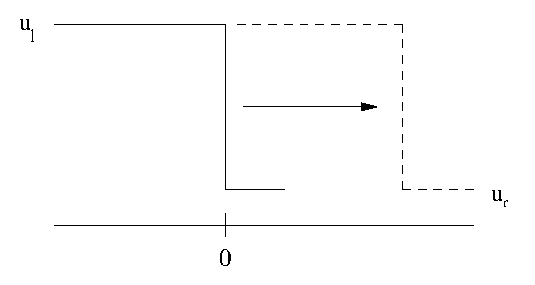
\includegraphics[scale=0.85]{figures/choc_choc.eps}\label{choc_choc}}
\hspace*{1cm}
\subfloat[Caractéristiques autour d'un choc]{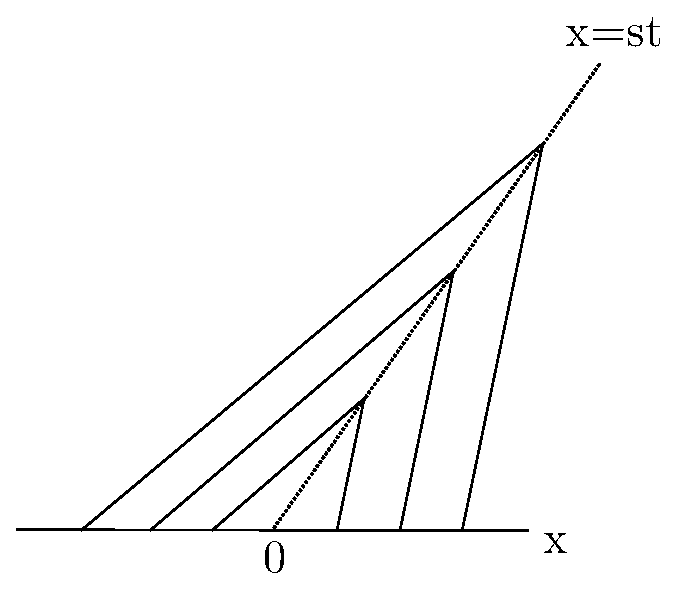
\includegraphics[scale=0.46]{figures/drawing.eps}\label{choc_caracteristiques}}
\caption{Choc - On remarque que les caractéristiques se dirigent vers le choc à mesure que le temps avance dans chaque région où $u$ est constant.}\label{figure_choc}
\end{figure}
%La figure \ref{choc_choc} illustre la propagation d'un choc, c'est-à-dire d'une discontinuité, sans déformation au cours du temps. Sur la figure \ref{choc_caracteristiques} est représenté le plan $x-t$ pour lequel on a tracé les caractéristiques dans une région proche d'un choc. On peut voir sur cette dernière que les caractéristiques semblent "rentrer" dans le choc.
\subsubsection{Cas d'une raréfaction : $v_l < v_r$}

Dans le cas où $v_l < v_r$, la solution faible n'est plus unique et il nous faut alors utiliser la condition d'entropie pour sélectionner celle qui est physiquement valide. Son énoncé, du à Oleinik \cite{oleinik1957discontinuous}, est le suivant 
\begin{theorem}
		$v(x,t)$ vérifie la condition d'entropie si toutes les discontinuités qu'elle contient vérifient la propriété que 
		\begin{equation}
			\frac{f(v) - f(v_l)}{v -v_l} \geq s \geq \frac{f(v) - f(v_r)}{v - v_r},
		\end{equation}
		pour tout $v$ compris entre $v_l$ et $v_r$.
\end{theorem}
On peut interpréter cette condition graphiquement à l'aide des caractéristiques. En effet, en prenant le cas de l'équation de Burgers pour exemple, si on trace les caractéristiques ainsi que le choc pour le cas précédent, comme sur la figure \ref{choc_caracteristiques}, on remarque que pour vérifier cette condition  les caractéristiques doivent être orientées vers le choc. 
Maintenant dans notre cas plusieurs solutions sont possibles dont le cas du choc avec $v_l<v_r$ (figure \ref{choc_rarefaction}), mais on voit graphiquement que cette dernière ne respecte pas la condition d'entropie puisque les caractéristiques sont orientées cette fois-ci vers l'extérieur du choc (voir figure \ref{choc_rarefaction_caracteristiques}). La solution physique est donnée par ce qu'on appelle une raréfaction qui vérifie la condition d'entropie et dont l'expression est donnée par
\begin{equation}
	v(x,t) =
	\left\{
		\begin{aligned}
			& v_l \quad & x<f'(v_l)t,\\
			& u(x/t)\quad & f'(v_l)t\leq x\leq f'(v_r)t,\\
			& v_r\quad & x> f'(v_r)t,
		\end{aligned}
	\right.
\end{equation}
avec $u(\xi)$ la solution de l'équation $f'(u(\xi)) = \xi$ appelée onde de raréfaction. Pour l'équation de Burgers, cela nous donne
\begin{equation}
	v(x,t) =
	\left\{
		\begin{aligned}
			& v_l \quad x<v_lt,\\
			& x/t\quad v_l t\leq x\leq v_r t,\\
			& v_r\quad x> v_r t.
		\end{aligned}
	\right.
\end{equation}
Nous avons tracé l'allure de la solution sur la figure \ref{rarefaction} ainsi que ses caractéristiques dans le plan $x-t$ sur la figure \ref{rarefaction_caracteristiques}. Nous voyons sur cette dernière que la condition d'entropie est cette fois bien vérifiée.

\begin{figure}\centering
\subfloat[Propagation d'un choc non-entropique]{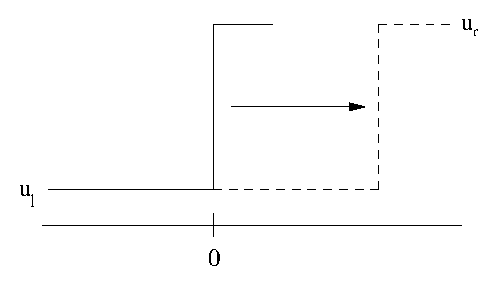
\includegraphics[scale=0.85]{figures/choc_rarefaction.eps}\label{choc_rarefaction}}
\hspace*{1cm}
\subfloat[Caractéristiques autour d'un choc non-entropique]{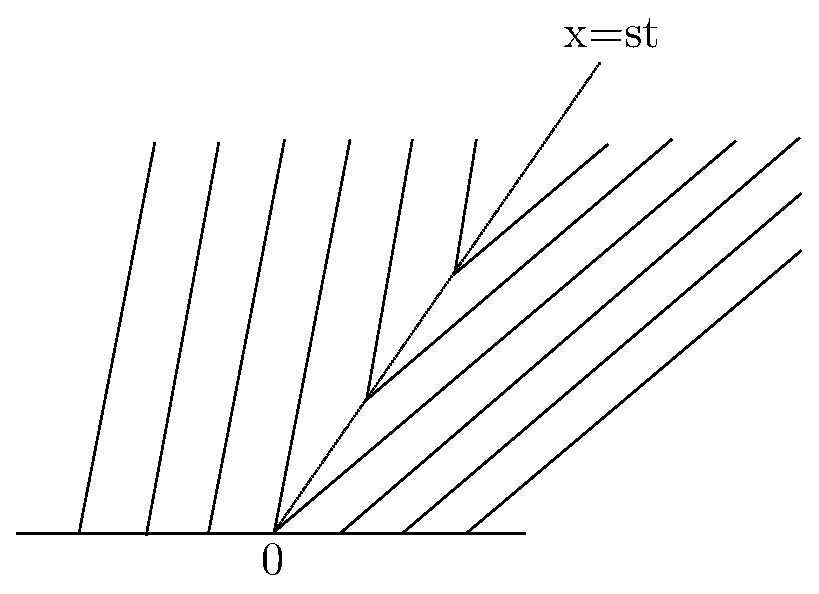
\includegraphics[scale=0.46]{figures/drawing2.eps}\label{choc_rarefaction_caracteristiques}}
\caption{Solution faible non-entropique - On remarque que les caractéristiques sont orientées vers l'extérieur du choc : la condition d'entropie n'est pas respectée.}\label{figure_choc_rarefaction}
\end{figure}

\begin{figure}[htb]\centering
\subfloat[Solution contenant une raréfaction]{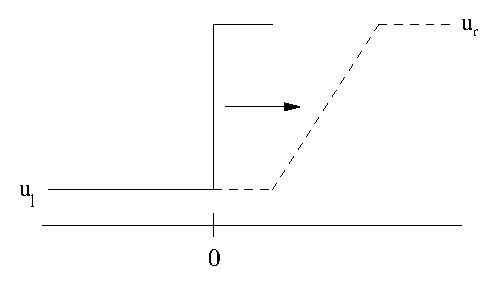
\includegraphics[scale=0.85]{figures/rarefaction.eps}\label{rarefaction}}
\hspace*{1cm}
\subfloat[Caractéristiques autour d'une zone de raréfaction]{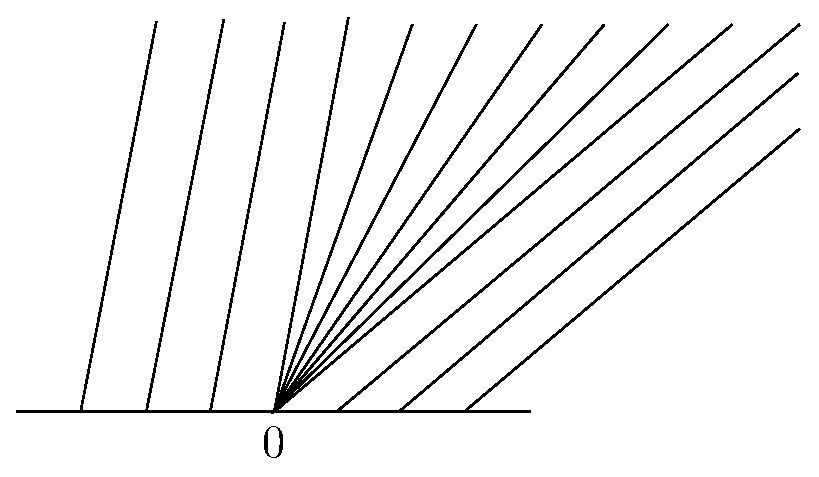
\includegraphics[scale=0.46]{figures/drawing3.eps}\label{rarefaction_caracteristiques}}
\caption{Raréfaction}\label{figure_rarefaction}
\end{figure}

\section{L'équation de Burgers relativiste}

Comme nous l'avons mentionné en introduction, l'équation de Burgers a été introduite pour modéliser les turbulences au sein d'un fluide. Toutefois, sa version sans viscosité \eqref{Burgers_standard} peut-être dérivée des \textbf{équations d'Euler}. Ceci est un point important, car c'est de cette manière que la \textbf{version relativiste} de l'équation peut être obtenue dans un espace-temps de Schwarzschild.

Les équations d'Euler décrivent la dynamique d'un fluide parfait, c'est-à-dire sans viscosité ni diffusion thermique. En une dimension, elles ont pour expression
\begin{equation}
	\frac{\partial}{\partial t} \begin{pmatrix}
 \rho \\
 \rho v \\
 E 
 \end{pmatrix} + \frac{\partial}{\partial x} \begin{pmatrix}
 \rho v \\
 \rho v^2 + p\\
 v \left(E + p\right) 
 \end{pmatrix} = 0,
\end{equation}
où $\rho$ est la densité, $v$ la vitesse, $\rho v$ la quantité de mouvement, $E$ l'énergie et $p$ la pression qui est fonction des autres variables. Elles peuvent s'écrire sous une forme tensorielle plus compacte à l'aide du tenseur énergie-impulsion pour un fluide parfait
\begin{equation}\label{tenseur_energie_impulsion_definition}
	T^{\alpha\beta} = \left(\rho + p\right) u^\alpha u^\beta + p g^{\alpha\beta},
\end{equation}
où $u =  (u^\alpha)$ est le champ de vecteur décrivant la vitesse au sein du fluide, que l'on prend normé. On le prend de plus comme étant de genre temps et orienté vers le futur. Ces propriétés se traduisent par la relation 
\begin{equation}
	u^\alpha u_\alpha = g_{\alpha\beta} u^\alpha u^\beta = -1,
\end{equation}
soit dans le cas d'une métrique diagonale\footnote{Les deux métriques auxquelles nous nous intéressons (Minkowski et Schwarzschild) étant diagonales, nous nous plaçons dans le cas d'une métrique diagonale quelconque tant qu'il est inutile de préciser laquelle des deux on utilise.} et à $1 + 1$ dimensions
\begin{equation}
	g_{00}(u^0)^2 + g_{11}(u^1)^2 = -1.
\end{equation}
Quant à $g^{\alpha\beta}$, ce sont les composantes de la métrique inverse, définie comme $g^{\alpha\gamma}g_{\gamma\beta} = \delta^\alpha_\beta$.
La forme tensorielle des équations d'Euler est alors donnée par
\begin{equation}
	\partial_\alpha T^{\alpha\beta} = 0.
\end{equation}
Cependant, cette équation n'est valable que dans le cas d'un espace plat et il faut pour pouvoir la généraliser à un espace courbe, remplacer les dérivées partielles par des dérivées covariantes
\begin{equation}\label{euler_courbe}
	\partial_\alpha T^{\alpha\beta} = 0 \rightarrow D_\alpha T^{\alpha\beta} = \partial_\alpha T^{\alpha\beta}
	+ \Gamma^\alpha_{\alpha\gamma} T^{\gamma\beta}
	+ \Gamma^\beta_{\alpha\gamma} T^{\alpha\gamma} = 0.
\end{equation}
Les coefficients $\Gamma^\gamma_{\alpha\beta}$ sont ce qu'on appelle les symboles de Christoffel. Ceux-ci contiennent l'effet de la courbure et peuvent s'exprimer en fonction de la métrique \cite{weinberg1972gravitation}
\begin{equation}
	\Gamma^{\gamma}_{\alpha\beta} = {\frac{1}{2}}g^{\gamma \delta}\left({\frac {\partial g_{\delta\beta}}{\partial x^{\alpha}}}+{\frac {\partial g_{\delta\alpha}}{\partial x^{\beta}}}-{\frac{\partial g_{\alpha\beta}}{\partial x^{\delta}}}\right).
\end{equation}
Pour pouvoir à présent dériver les deux équations à partir de la relation \eqref{euler_courbe}, il faut se placer dans le cas d'un fluide sans pression, soit $p=0$. Les équations d'Euler se simplifient et deviennent
\begin{equation}
	D_\alpha \left(\rho u^\alpha u^\beta\right) = 0.
\end{equation}
On définit ensuite la quantité $v$ comme
\begin{equation}\label{definition_v}
	v := - \frac{1}{g_{00}} \frac{u^1}{u^0}
\end{equation}
et on réécrit les composantes du champ de vitesse en fonction de cette nouvelle quantité :
\begin{equation}
  \left\{
      \begin{aligned}
        (u^0)^2 & = -\frac{1}{g_{00}(1+g_{00}g_{11}v^2)},\\
        (u^1)^2 & = -\frac{g_{00}v^2}{1+g_{00}g_{11}v^2}.
      \end{aligned}
    \right.
\end{equation}
Cela nous permet finalement de pouvoir réécrire le tenseur énergie-impulsion en fonction de $v$ en injectant les relations précédentes dans son expression \eqref{tenseur_energie_impulsion_definition}. En regroupant ses composantes dans une matrices $2\times 2$, il s'écrit :
\begin{equation}
\begin{pmatrix}\label{tenseur_energie_impulsion}
	T^{00} & T^{01} \\
	T^{10} & T^{11} 
\end{pmatrix}
=
\begin{pmatrix}
	-\frac{\rho}{g_{00}(1+g_{00}g_{11}v^2)}   & -\frac{\rho v}{g_{00}(1+g_{00}g_{11}v^2)} \\
	-\frac{\rho v}{g_{00}(1+g_{00}g_{11}v^2)} & -\frac{g_{00}\rho v^2}{1+g_{00}g_{11}v^2}
\end{pmatrix}.
\end{equation}

\subsection{Dérivation de l'équation standard}

Maintenant que nous avons introduit tout les prérequis nécessaires, nous pouvons obtenir l'équation de Burgers standard en se plaçant dans le cas de la \textbf{métrique plate de Minkowski} $(\eta_{\alpha\beta}) = \mathrm{diag}(-1,+1,+1,+1)$. Toutes les dérivées covariantes sont alors de simples dérivées partielles ($D_\alpha = \partial_\alpha$), puisque les symboles de Christoffel sont tous nuls. En remplaçant de plus $g_{00}$ et $g_{11}$ par leurs expressions dans \eqref{tenseur_energie_impulsion} et en injectant le résultat dans les équations d'Euler on obtient
\begin{align}
	\beta = 0 : \quad\partial_0 T^{00} + \partial_1 T^{10} = \partial_t (\frac{\rho}{1- v^2}) + \partial_r (\frac{\rho v}{1 - v^2}) = 0, \\
	\beta = 1 : \quad\partial_0 T^{01} + \partial_1 T^{11} = \partial_t (\frac{\rho v}{1 - v^2}) + \partial_r(\frac{\rho v^2}{1- v^2}) = 0.
\end{align}
En réécrivant l'équation pour $\beta = 1$
\begin{equation}
	v\partial_t (\frac{\rho }{1 - v^2}) + \frac{\rho }{1 - v^2}\partial_t v + v\partial_r(\frac{\rho v}{1- v^2}) + \frac{\rho v}{1- v^2}\partial_r v = 0,
\end{equation}
et en soustrayant l'équation pour $\beta = 0$ multipliée par $v$, on obtient enfin l'équation de Burgers standard \eqref{Burgers_standard}.

\subsection{L'équation relativiste}

De manière analogue, on va obtenir l'équation relativiste en se plaçant dans le cas de la \textbf{métrique de Schwarzschild}. Néanmoins, les symboles de Christoffel ne sont pas tous nuls et nous avons
%\begin{equation}
\begin{eqnarray}
		\Gamma^{t}_{tr} &=& \Gamma^{t}_{rt} =
						  - \frac{M}{r^2}\left(1-\frac{2M}{r}\right)^{-1} \qquad
		\Gamma^{r}_{tt} = \frac{M}{r^2}\left(1-\frac{2M}{r}\right) \qquad
		\Gamma^{r}_{rr} = -\frac{M}{r^2}\left(1-\frac{2M}{r}\right)^{-1} \\
		\Gamma^{r}_{\theta\theta} &=& -r\left(1-\frac{2M}{r}\right) \qquad\qquad\qquad\:\:
		\Gamma^{r}_{\phi\phi} = -r\sin^2\theta\left(1-\frac{2M}{r}\right) \\
		\Gamma^{\theta}_{r \theta} &=& \Gamma^{\theta}_{\theta r}  = \frac{1}{r} \qquad\qquad\qquad\qquad\quad\:\:\:
		\Gamma^{\theta}_{\phi\phi} = -\sin\theta\cos\theta \quad\qquad
		\Gamma^{\phi}_{r\phi} = \Gamma^{\phi}_{\phi r}  = \frac{1}{r} \\
		\Gamma^{\phi}_{\theta\phi} &=& \Gamma^{\phi}_{\phi\theta}  = \cot \theta.
\end{eqnarray}
%\end{equation}
En injectant alors leurs expressions dans les équations d'Euler, et en remplaçant également  $g_{00}$ et $g_{11}$ par leurs expressions dans \eqref{tenseur_energie_impulsion}, on a
\begin{align}
	\beta = 0 : \quad\partial_t(\frac{r^2 \rho }{1 - v^2}) + \partial_r(r(r-2M)\frac{\rho v}{1-v^2}) = 0,\\
	\beta = 1 : \quad\partial_t (\frac{r^2\rho v}{1 - v^2}) + \partial_r(r(r-2M)\frac{\rho v^2}{1 - v^2}) = -M\rho.
\end{align}
Comme pour l'équation standard, on réécrit l'équation pour $\beta =1$
\begin{equation}
	v\partial_t(\frac{r^2\rho v}{1 - v^2}) + \frac{r^2\rho v}{1 - v^2} \partial_t v + v, \partial_r(r(r-2M)\frac{\rho v}{1-v^2}) + r(r-2M)\frac{\rho v}{1-v^2}\partial_r v = -M\rho,
\end{equation}
puis en soustrayant l'équation $\beta = 0$ multipliée par $v$ on obtient l'équation de Burgers relativiste dans un espace-temps de Schwarzschild
\begin{equation}
	\partial_t v + \left(1 - \frac{2M}{r}\right)\partial_r\left(\frac{v^2}{2}\right) = \frac{M}{r^2}\left(v^2 -1\right).
\end{equation}
On peut aller plus loin en écrivant cette équation sous une forme conservative \eqref{loi_de_conservation}. Pour la voir apparaître,  il suffit de réécrire l'équation selon
\begin{equation}
	\partial_t v + \left(1 - \frac{2M}{r}\right)\partial_r\left(\frac{v^2-1}{2}\right) - \frac{2M}{r^2}\left(\frac{v^2 -1}{2}\right) = 0,
\end{equation}
où l'on voit apparaître la dérivée par rapport à $r$ du rapport de deux fonctions si l'on divise l'équation par $\left(1-\frac{2M}{r}\right)^2$. On obtient finalement la forme conservative de l'équation :
\begin{equation}\label{Burgers_relativiste_conservative}
	\partial_t \left(\frac{v}{(1-\frac{2M}{r})^2}\right) + \partial_r\left(\frac{v^2-1}{2\left(1-\frac{2M}{r}\right)}\right) = 0.
\end{equation}
Cette équation va nous être utile par la suite pour définir des méthodes numériques conservatives et notamment la méthode de Lax-Friedrichs.
On finira par remarquer qu'en faisant tendre la masse du trou noir $M \to 0$ dans \eqref{Burgers_relativiste_conservative}, on retrouve bien l'équation de Burgers standard 
\begin{equation}\label{standard}
\partial_t v+  \partial_r  \Big({ v^2\over2 } \Big)=0. 
\end{equation}

\subsection{Solutions statiques}

Une classe de solutions importantes du modèles de Burgers relativiste sont ses \textbf{solutions statiques}. En effet, elles rentrent dans la définition du \textbf{problème de Riemann généralisé}, que nous décrirons plus tard et qui est lui-même important dans la définition de la \textbf{méthode de Glimm généralisée}.

\subsubsection{Résolution de l'équation statique}
Pour trouver l'expression de ces solutions statiques, que l'on notera $v_*$, il nous faut résoudre l'équation de Burgers relativiste indépendante du temps, soit
\begin{equation}
	\frac{\mathrm{d}}{\mathrm{d}r}\left(	\frac{v_*^2 -1}{2\left(1-\frac{2M}{r}\right)}\right) = 0.
\end{equation}
Si pour un rayon donné $r=r_0$, la solution vaut $v(r_0) = v_0$, l'intégration de l'équation précédente nous donne la relation suivante
\begin{equation}
\frac{v_*^2-1}{1-\frac{2M}{r}} = \frac{v_0^2 - 1}{1 - \frac{2M}{r_0}}.
\end{equation}
On défini alors le paramètre positif $K_*(r_0, v_0) := \sqrt{\frac{1 - v_0^2}{1 -\frac{2M}{r_0}}}$ et on obtient après réarrangement de l'équation précédente
\begin{equation}
	v_*^2 = 1 - \left(1-\frac{2M}{r}\right)K_*^2(r_0,v_0).
\end{equation}
En conclusion, pour une vitesse $v_0$ donnée au rayon $r = r_0 > 2M$, l'équation de Burgers relativiste indépendante du temps admet pour solution unique 
\begin{equation}\label{solution_statique}
	v_*(r) = \text{sgn}(v_0) \sqrt{1 - K_*^2\left(1 - \frac{2M}{r}\right)}.
\end{equation}
Nous avons représenté plusieurs de ces solutions statiques en \ref{courbe_solution_statique}, avec une valeur de $K_*$ différente à chaque fois.

\subsubsection{Domaine de définition de la solution}\label{domaine_definition}

Comme dit précédemment nous voulons étudier les solutions du modèle de Burgers relativiste sur le \textbf{domaine extérieur} du trou noir de Schwarzschild, soit $r\in ]2M,+\infty[$. Cependant, d'après l'expression de la solution statique \eqref{solution_statique}, celle-ci n'est pas forcément définie sur tout ce domaine. En effet, si dans cette expression l'argument de la racine devient négatif, la solution va alors cesser d'exister. Le terme $1 -\frac{2M}{r}$ étant compris dans l'intervalle $]0,1[$, cela va donc dépendre du signe de la quantité $1 - K_*$. Dans le cas où $K_*<1$, la solution est définie sur tout le domaine extérieur mais dans le cas où $K_*>1$, l'argument s'annule pour un certain rayon $r = r^\natural$ et devient négatif pour $r> r^\natural$. Ces deux possibilités sont séparées par le cas critique où $K_*=1$ c'est à dire $|v_0| = \sqrt{\frac{2M}{r_0}}$. Ainsi d'après ce qui précède, c'est la donnée du point $(r_0, v_0)$ que l'on se fixe qui détermine si la solution est définie sur tout le domaine ou bien sur une partie seulement. Cela motive l'introduction des deux solutions stationnaires critiques $v^\pm_{**} = v^\pm_{**}(r)$ ayant pour expression
\begin{equation}
v^\pm_{**}(r) := \pm\sqrt{\frac{2M}{r}},
\end{equation}
puisque le graphe de ces courbes sépare l'ensemble possible des valeurs de la vitesse $[-1,1]$\footnote{On rappelle qu'on s'est placé dans le cas où $c=1$.} en trois domaines disjoints : $[-1,v_{**}^-(r)],\, ]v_{**}^-,v_{**}^+[,\, [v_{**}^+, 1]$. Cela nous permet de définir l'ensemble des grandes vitesses par $\mathcal{G} :=[-1,v_{**}^-(r)] \cup[v_{++}^+, 1]$ et l'ensemble des petite vitesse par $\mathcal{P} = ]v_{**}^-,v_{**}^+[$. Ainsi, si $v_0\in\mathcal{G}$ (ou autrement dit si $0\leq K_*(r_0,v_0) \leq 1$), la solution statique peut-être définie sur tout le domaine extérieur tandis que si $v_0\in\mathcal{P}$ (autrement dit si $K_*(r_0,v_0) > 1$), elle ne peut-être définie que sur la portion $]2M, r^\natural[$. Dans le cas des petites vitesses, le rayon d'annulation de la solution statique $r=r^\natural$ a pour expression\footnote{Pour une démonstration, voir \cite{PLF-SX-one}.}
\begin{equation}\label{rayon_annulation}
	r^\natural := \frac{2MK_*^2}{K_*^2 -1}.
\end{equation}

%	Soit la vitesse de la lumière $c=1$ et la masse du trou noir $M>0$, nous considérons le modèle de Burgers statique décrivant l'écoulement d'un fluide dans un espace-temps de Schwarzschild.

\subsubsection{Propriétés des solutions statiques}

Les \textbf{solutions statiques}, dont le domaine de définition est fixé par $v_0$, possèdent une première propriété importante. En effet, pour une solution statique $v_* = v_*(r)$, l'intervalle $]2M, r_0[$ sera toujours contenu dans le domaine de définition, indépendamment de la valeur de $v_0$, ceci d'après \eqref{rayon_annulation}. Autrement dit, nous pouvons au moins garantir l'existence d'une solution statique à gauche du point $r=r_0$. Cette propriété sera importante lorsque l'on s'intéressera plus tard au schéma de Glimm généralisé.

Les solutions vérifient de plus, en fonction de la valeur de $v_0$, des propriétés de monotonicité et de convexité sur leur domaine de définition.
\begin{itemize}
\item Si $v_0 \in \mathcal{G}$ et si de plus $v_0 < 0$ (resp. $v_0> 0$), alors la solution sera croissante (resp. décroissante) et concave (resp. convexe).
\item Si $v_0 \in \mathcal{P}$, deux cas se présentent :
	\subitem Quand $1 < K_*\leq 2$ et que $v_0 >0$ (reps. $v_0<0$), alors la solution $v_*$ est convexe (resp. concave) sur $]2M, r^\sharp[$ et concave (resp. convexe) sur $]r^\sharp,r^\natural[$ si $v_0 > 0$. Ici, le rayon $r=r^\sharp$ est donné par
\begin{equation}
	r^\sharp := \frac{3MK_*^2}{2\left(K_*^2-1\right)}.
\end{equation}
	\subitem Quand $K_* > 2$, $v_*$ est concave sur $]2M, r^\natural[$ si $v_0>0$ et convexe si $v_0<0$.
\end{itemize}

Enfin, on a les valeurs limites suivantes
\begin{itemize}
\item Si $v_0 \in \mathcal{G}$ :
\begin{equation}
	\lim\limits_{r\rightarrow 2M} v_*(r) = sgn(v_0), \qquad \lim\limits_{r\rightarrow +\infty} v_*(r) = sgn(v_0)\sqrt{1 - K_*^2},
\end{equation}
\item Si $v_0 \in \mathcal{P}$ :
\begin{equation}
	\lim\limits_{r\rightarrow 2M} = \text{sgn}(v_0),\qquad \lim\limits_{r\rightarrow r^\natural} v_*(r) = 0, \qquad \lim\limits_{r\rightarrow r^\natural} \frac{\mathrm{d}v_*}{\mathrm{d}r} = -\text{sgn}(v_0)\infty.
\end{equation}
\end{itemize}

\begin{figure}\centering
\subfloat[Solutions statiques]{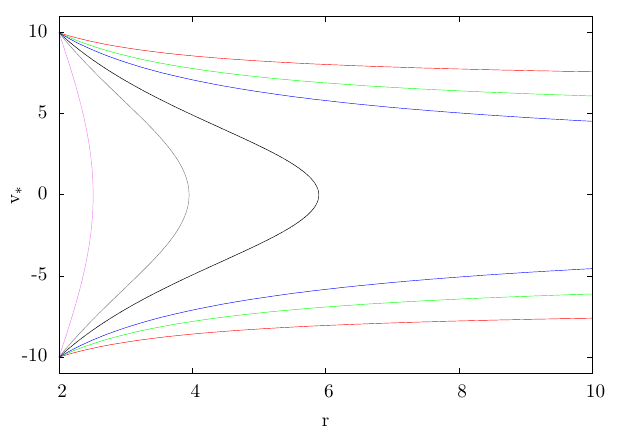
\includegraphics[scale=0.45]{figures/solution_statique.png}\label{courbe_solution_statique}}
\hspace*{1cm}
\subfloat[Domaines de vitesse]{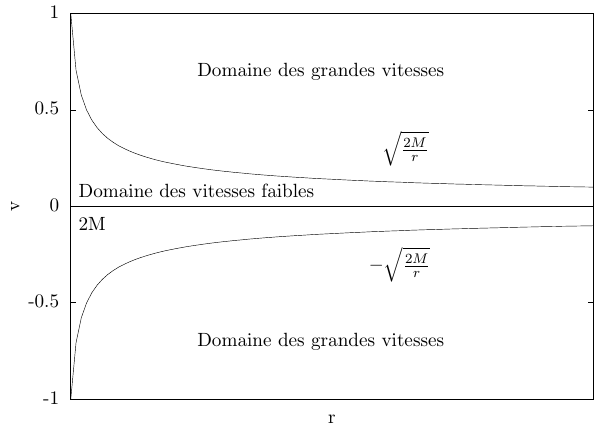
\includegraphics[scale=0.45]{figures/pastedImage.png}\label{domaines}}
\caption{Sur la figure \ref{courbe_solution_statique}, nous avons tracé plusieurs solutions statiques pour une valeur de $K_*$ différente à chaque fois. La figure \ref{domaines} illustre quant elle les différents domaines de vitesse que l'on a introduit.}\label{figure_solution_statique}
\end{figure}

\subsection{Le problème de Riemann généralisé}

Le problème de Riemann que nous avons introduit plus tôt, ne peut pas être appliqué tel quel à l'équation de Burgers relativiste. Or, comme nous l'avons déjà mentionné, sa résolution est indispensable pour la définition de la méthode de Glimm. 

La condition initiale qui consistait toute à l'heure en deux états constants séparés par une discontinuité en $r = r_0$, doit être modifiée car les états constants ne sont plus des états stationnaires de l'équation relativiste. En d'autres termes, nous allons remplacer les deux états constants $u_l$ et $u_r$ par deux \textbf{solutions statiques} que nous noterons $v_L(r)$ et $v_R(r)$ et dont l'expression est donnée en \eqref{solution_statique}. Le \textbf{problème de Riemann généralisé}, va donc consister à résoudre l'équation de Burgers relativiste \eqref{Burgers_relativiste_conservative} pour la donnée initiale
\begin{equation}
	v(r,t) =
	\left\{
		\begin{aligned}
			& v_L(r) \quad r< \sigma(t), \\
			& v_R(r)\quad r> \sigma(t),
		\end{aligned}
	\right.
\end{equation}
où $[\bar{r}, \hat{r}] \subset ]2M,+\infty[$ est le domaine sur lequel on restreint notre étude. Les solutions statiques s'écrivent 
\begin{equation}
	v_L(r) = \text{sgn}(v_L^0)\sqrt{1 - K_L^2\left(1-\frac{2M}{r}\right)}, \quad v_R(r)= \text{sgn}(v_R^0)\sqrt{1 - K_R^2\left(1-\frac{2M}{r}\right)},
\end{equation}
avec $K_L = K(r_0, v_L^0)$ et $K_R = K(r_0, v_R^0)$ où $v_L^0 = v_L(r_0)$ et $v_R^0 = v_R(r_0)$. De manière analogue au cas standard, nous avons deux types de solutions selon la relation entre $v_L^0$ et $v_R^0$ : soit un choc si $v_L^0 > v_R^0$, soit une raréfaction si $v_R^0 > v_L^0$. Cependant, comme nous l'avons mentionné plus tôt, le choc ainsi que les caractéristiques ne seront plus des droites dans le plan $r-t$ mais des fonctions plus compliquées. Nous ne faisons ici qu'énoncer les résultats dont la démonstration peut-être trouvée dans \cite{PLF-SX-one}, \cite{lefloch2016weakly}.

\subsubsection{Cas d'un choc}

Pour commencer, la vitesse du choc va être modifiée par la géométrie et celle-ci va alors dépendre de $r$. En utilisant la condition d'Hugoniot-Rankine \eqref{hugoniot_rankine_condition} on trouve
\begin{equation}
	s(r) = \left(1-\frac{2M}{r}\right)\frac{v_L(r)+v_R(r)}{2},
\end{equation}
qui nous redonne comme à chaque fois le cas standard en faisant tendre la masse $M$ vers $0$. Nous pouvons alors à partir de l'expression de sa vitesse, trouver son expression que l'on note $\sigma(t)$, en intégrant l'EDO
\begin{equation}
	\frac{\mathrm{d}\sigma}{\mathrm{d}t} = \left(1 - \frac{2M}{\sigma}\right) \frac{v_L(\sigma) + v_R(\sigma)}{2}.
\end{equation}
Après intégration, nous obtenons l'équation non-linéaire suivante à résoudre 
\begin{equation}
R_S(\sigma (t);  v_L, v_R)-  R_S(r_0;  v_L, v_R)= t,
\end{equation}
où la fonction $R_S= R_S(r; v_L, v_{R})$ est définie par  
  \begin{equation}\label{speed-3}
 \aligned 
  R_S(r,  v_L, v_{R})=&  \text{sgn}(v_L+ v_{R}) {2 \over {K_{*}^R}^2-{K_*^L}^2  } \Bigg( {r-4M \over r-2M }\Bigg(\sqrt {{1}- {K_*^L}^2\Big(1- {2M\over r}\Big) } -  \sqrt {{1}- {K_{*}^R}^2\Big(1- {2M\over r}\Big) }\Bigg )
 \\
 & - M({4}- 3{K_{*}^R}^2  )\bigg(  \ln \Big( r \sqrt {{1}- {K_*^L}^2}   \sqrt {{1}- {K_{*}^R}^2 \Big(1- {2M\over r}\Big)  } + ( M-r) {K_{*}^R}^2+{ r}  \Big )
 \\
& +\ln  \Big( {2 r \over (r-2M)}  \sqrt {{1}- {K_{*}^R}^2 \Big(1- {2M\over r}\Big)}- {K_{*}^R}^2\Big )\bigg)
\\
& + M({4}- 3{K_*^L}^2  )\bigg(  \ln \Big( r \sqrt {{1}- {K_*^L}^2}   \sqrt {{1}- {K_*^L}^2 \Big(1- {2M\over r}\Big)  } + ( M-r) {K_*^L}^2+{ r}  \Big )
 \\
& -\ln  \Big( {2 r \over (r-2M)}  \sqrt {{1}- {K_*^L}^2 \Big(1- {2M\over r}\Big)}- {K_*^L}^2\Big )\bigg)
\Bigg), 
 \endaligned 
\end{equation}
avec ${K_*^L}^2= {1 -v_L^2\over (1-2M/r)}$ et $ {K_{*}^R}^2= {1-v_{R}^2\over (1-2M/r)}$.
Dans le cas du choc, la solution a pour expression
\begin{equation}\label{solution_choc}
	v(r,t) = \left\{
	\begin{aligned}
	             &v_L(r)\quad \bar{r} <r< \sigma(t)\\
			     &v_R(r)\quad \hat{r} > r> \sigma(t)
			     \end{aligned}
			\right.
\end{equation}

\subsubsection{Cas d'une raréfaction}

Pour le cas de la raréfaction, comme nous l'avons dit, les caractéristiques ne sont plus des droites et donc $u_l t$ et $u_r t$ qui délimitaient la zone de raréfaction pour le problème de Riemann standard sont remplacées par les courbes $\sigma_L(t)$ et $\sigma_R(t)$.
Ces deux courbes satisfont comme pour $\sigma(t)$, une EDO à intégrer
\begin{equation}
	\frac{\mathrm{d}\sigma_L}{\mathrm{d}t} = \left(1 - \frac{2M}{\sigma_L}\right) v_L(\sigma_L)\quad \text{et} \quad \frac{\mathrm{d}\sigma_R}{\mathrm{d}t} = \left(1 - \frac{2M}{\sigma_R}\right) v_R(\sigma_R),
\end{equation}
qui nous donne pour chacune une équation non-linéaire à résoudre. Pour $\sigma_L (t)$, on a 
\begin{equation}
R_L(\sigma_L (t), v_L)- R_L(r_0, v_L)= t, 
\end{equation}	
où la fonction $R_L= R(r, v_L )$ est donnée par
\begin{equation}\label{speed-1}
\aligned 
 R_L (r, v_L) : = & \text{sgn}(v_L)\frac{1}{(1 - {K_*^L}^2 )^{3/2}} 
\Bigg (  2 M \big({1}  - {K_*^L}^2\big)^{3/2} \ln (r- 2M )
\\  
& -2M  \big({1}  - {K_*^L}^2\big)^{3/2} \ln \Big( {2 r}  \sqrt {{1}- {K_*^L}^2 \Big(1- {2M\over r}\Big)} +( 2M-r) {K_*^L}^2\Big )
\\
& 
+ r \sqrt {{1}  -{K_*^L}^2}   \sqrt {{1}- {K_*^L}^2\Big(1- {2M\over r}\Big) } 
\\
& + M(2 -3 {K_*^L}^2 ) \ln \Big( r \sqrt {{1}- {K_*^L}^2}   \sqrt {{1}- {K_*^L}^2 \Big(1- {2M\over r}\Big)  } + ( M-r) {K_*^L}^2+{ r}  \Big )
 \Bigg), 
 \endaligned 
\end{equation}
avec ${K_*^L}^2$ ayant la même expression que dans le cas du choc. 
Quant à $\sigma_R(t)$, elle vérifie l'équation non-linéaire
\begin{equation}
R_R(\sigma_R (t), v_R)- R_R(r_0, v_R)= t, 
\end{equation}
où $R_R = R_R(r, v_R)$ est donnée par
\begin{equation}
\aligned 
 R_R (r, v_R) : = & \text{sgn}(v_R)\frac{1}{(1 - {K_*^R}^2 )^{3/2}} 
\Bigg (  2 M \big({1}  - {K_*^R}^2\big)^{3/2} \ln (r- 2M )
\\  
& -2M  \big({1}  - {K_*^R}^2\big)^{3/2} \ln \Big( {2 r}  \sqrt {{1}- {K_*^R}^2 \Big(1- {2M\over r}\Big)} +( 2M-r) {K_*^R}^2\Big )
\\
& 
+ r \sqrt {{1}  -{K_*^R}^2}   \sqrt {{1}- {K_*^R}^2\Big(1- {2M\over r}\Big) } 
\\
& + M(2 -3 {K_*^R}^2 ) \ln \Big( r \sqrt {{1}- {K_*^R}^2}   \sqrt {{1}- {K_*^R}^2 \Big(1- {2M\over r}\Big)  } + ( M-r) {K_*^R}^2+{ r}  \Big )
 \Bigg), 
 \endaligned 
\end{equation}
avec ${K_*^R}^2$ ayant la même expression que dans le cas du choc.
Pour finir, l'expression de l'onde de raréfaction $w(t,r)$ va être aussi modifiée et avoir pour expression
\begin{equation}\label{curved-ra}
w(t, r) = \text{sgn}(r-r_0 )  \sqrt{{1} -K^2 (t,r ) \Big(1-{ 2M \over r}\Big)},  
\end{equation}
où $K  = K (t,r )>0 $  est une fonction de $t>0$ et de $r>2M$ satisfaisant l'égalité
\begin{equation}\label{K_*}
 \text{sgn}(r-r_0 )   {R(r, K)-R(r_0, K) \over t} =1, 
\end{equation}
avec la fonction $R= R(r, K)$ donnée par
\begin{equation}\label{Rcurve}
\aligned 
R(r, K): & ={1  \over (1 - K^2 )^{3/2}}  \Bigg (  2 M  \big({1}  - K^2\big)^{3/2} \ln (r- 2M )
\\  
& -2M  \big({1}  - K ^2\big)^{3/2} \ln \Big( {2 r}  \sqrt {{1}- K ^2 \Big(1- {2M\over r}\Big)} +( 2M-r) K ^2\Big )
\\
& 
+\bigg(r \sqrt {{1}  - K ^2}   \sqrt {{1}- K  ^2\Big(1- {2M\over r}\Big) } 
\\
& + M \big ({2} -3 K ^2 ) \ln \Big( r \sqrt {{1}- K ^2}   \sqrt {{1}- K ^2 \Big(1- {2M\over r}\Big)  } + ( M-r) K ^2+{r}  \Big )
 \bigg) 
 \Bigg). 
\endaligned 
\end{equation}
Dans le cas du choc, la solution a pour expression
\begin{equation}\label{solution_rarefaction}
	v(r,t) = \left\{
	\begin{aligned}
	             &v_L(r)\quad \bar{r} < r< \sigma_L(t),\\
	             & w(t,r) \quad\sigma_L(t) \leq r \leq \sigma_R(t),\\
			     &v_R(r)\quad \hat{r} > r > \sigma_R(t).
			     \end{aligned}
			\right.
\end{equation} 
Nous pouvons réécrire les deux solutions \eqref{solution_choc} et \eqref{solution_rarefaction} sous la forme d'une équation générale qui rassemble ces deux cas : 
 \begin{equation}\label{Riemann-sol}
v(t, r)= 
\begin{cases}
v_L(r)&  \bar r<r< \sigma_-( t) , \\ 
w(t,r) & \sigma_-(t) < r < \sigma_+(t),\\
v_R(r) &  \sigma_+ (t) < r <\hat r, 
\end{cases}
\end{equation}
où
\begin{equation}\label{region}
\sigma_-(t) = \begin{cases}
\sigma (t) ,  & v_L^0>v_R^0,\\
\sigma_ L (t),  & v_R^0>v_L^0, 
\end{cases} 
\qquad 
\sigma_+ (t)= \begin{cases}
\sigma (t) ,  & v_L^0>v_R^0,\\
\sigma_R  (t) ,  & v_R^0>v_L^0. 
\end{cases}
\end{equation}
\`{A} noter que l'on retrouve tous les résultats du cas standard \ref{probleme_riemann_standard} en faisant tendre la masse du trou noir $M\rightarrow 0$.

\section{Méthodes numériques}

\`{A} présent que nous avons introduit l'équation de Burgers dans sa version \textbf{standard} \eqref{Burgers_standard} et \textbf{relativiste} \eqref{Burgers_relativiste_conservative}, nous allons nous intéresser à la résolution numérique de cette deuxième avec une \textbf{méthode de Lax-Friedrichs et de Glimm}. Dans les deux cas, nous discrétisons le plan $r-t$ avec $\Delta t$, le pas en temps, et $\Delta r$, le pas en espace, tous deux constants. Les points $(r_j, t_n)$ du maillage sont alors définis par
\begin{align}
	&r_j = 2M + j \Delta r, \quad j\in\mathbb{N^+}\\
	&t_n = n\Delta t, \quad n \in \mathbb{N}^+.
\end{align}
%Nous présenterons donc à chaque fois la méthode numérique dans sa forme standard avant de présenter sa généralisation au cas relativiste. Nous ne listons ici que des méthodes dites conservatives. Certaines méthodes comme la discrétisation des dérivées ne convergera pas et c'est pourquoi nous nous intéressons à celle-ci. Le fait que la solution soit discontinue pose problème en plus du fait que l'équation n'est pas linéaire.

\subsection{La Méthode de Lax-Friedrichs}

La méthode de Lax-Friedrichs est une méthode numérique dite conservative, c'est-à-dire qu'elle s'écrit sous la forme
\begin{equation}\label{methode_conservative}
	U^{n+1}_j = U_j^n - \frac{\Delta t}{\Delta r}\left[F\left(U^n_j, U^n_{j+1}\right) - F\left(U^n_{j-1}, U^n_j\right)\right],
\end{equation}
où $U^n_j$ est l'approximation de la solution de l'EDP au point $r_j$ et au temps $t_n$. Quant à $F$, elle est ce qu'on appelle la fonction de flux numérique. Dans le cas de Lax-Friedrichs appliqué au modèle de Burgers standard, elle a pour expression \cite{leveque1992numerical} 
\begin{equation}
	F\left(U_j^n, U^n_{j+1}\right) = \frac{\Delta r}{2\Delta t}\left(U^n_j - U^n_{j+1}\right) + \frac{1}{2}\left(f(U^n_j) + f(U^n_{j+1})\right),
\end{equation}
avec $f(u)= \frac{u^2}{2}$.

On veut maintenant dériver une \textbf{méthode de Lax-Friedrichs} pour l'équation de Burgers relativiste \eqref{Burgers_relativiste_conservative}.

\subsubsection{Dérivation de la méthode}

La relation algébrique \eqref{methode_conservative} étant valable pour n'importe quelle méthode conservative, c'est donc le flux numérique qui va différer de celui du cas standard.
Dans le but de trouver son expression, nous modifions l'équation relativiste dans sa forme conservative \eqref{Burgers_relativiste_conservative} en posant
 \begin{equation}\label{w_expr}
w = \frac{v}{(1-\frac{2M}{r})^2} , 
\end{equation}
ce qui nous donne une fois l'équation réécrite en terme de cette nouvelle fonction $w$ : 
\begin{equation}\label{Burgers_w''}
\partial_tw + \partial_r\left(\frac{\left(1-2M/ r\right)^4w^2 - 1}{2\left(1-2M/ r\right)}\right)=0. 
\end{equation}
En intégrant \eqref{Burgers_w''} de $r_{j-1/2}$ à $r_{j+1/2}$ en espace et de $t_n$ à $t_{n+1}$ en temps, on a :
\[ 
\int_{r_{j-1/2}}^{r_{j+1/2}}
	\int_{t_n}^{t_{n+1}}
		\partial_t w 
	\,\mathrm{d}r
\mathrm{d}t
+\int_{r_{j-1/2}}^{r_{j+1/2}}
	\int_{t_n}^{t_{n+1}}
		\partial_r\left(
			\frac{\left(1-2M/r\right)^4 w^2-1}{2\left(1-2M/r\right)}
				  \right)
	\,\mathrm{d}r
\mathrm{d}t
= 0, 
\]
ce qui nous donne 
\[
\aligned 
\int_{r_{j-1/2}}^{r_{j+1/2}}
	\left(
		w(t_{n+1},r)-w(t_n,r)
	\right) 
\,\mathrm{d}r
+ 
\int_{t_n}^{t_{n+1}}
	\left[
		\left(
			1-\frac{2M}{r_{j+1/2}}
		\right)^3
		\frac{w^2(t,r_{j+1/2})}{2}
		-\frac{1}{2\left(1-\frac{2M}{r_{j+1/2}}\right)}
	\right. \\
	\left.
		-\left(
			1-\frac{2M}{r_{j-1/2}}
		\right)^3
		\frac{w^2(t,r_{j-1/2})}{2}
		+\frac{1}{2\left(1-\frac{2M}{r_{j-1/2}}\right)}
	\right]
\,\mathrm{d}t \nonumber
= 0.
\endaligned 
\] 
Soit $W_j^n$ la valeur moyenne en espace de la solution dans le sens où 
\begin{equation}\label{W}
W_j^n : =  {1\over h}\int_{r_{j-1/2}}^{r_{j+1/2}}
w(t_{n+1},r)	
\,\mathrm{d}r, 
\end{equation}
on peut alors en déduire que la méthode de Lax-Friedrichs pour le modèle de Burgers relativiste :
\begin{equation}\label{Lax-Friedrichs}
W_j^{n+1} =   W_j^n
            - \frac{k}{h}\left(F_{j+1/2}^n- F_{j-1/2}^n
 \right) \nonumber,		    
\end{equation}
où le flux numérique $F^n_{j+1/2}$ est donné par
\begin{equation}\label{rnff}
	F_{j + 1/2}^n
	=
	  \left(
          1-\frac{2M}{r_{j + 1/2}}
      \right)^3 F_s(W_j^n,W_{j + 1}^n) 
    - \frac{1}{2\left(1-\frac{2M}{r_{j+ 1/2}}\right)},
\end{equation}
avec $F_s$ défini comme
\begin{equation}\label{F_c}
F_s(W_j^n,W_{j+1}^n)
= \frac{f_s(W_j^n) + f_s(W_{j+1}^n)}{2}-\frac{h}{2k}(W_{j+1}^n-W_j^n). 
\end{equation}

On remarque que $F_s$ représente le flux numérique dans le modèle de Burgers standard \eqref{standard}. 

\subsubsection{La propriété de consistance}
 
On veut à présent montrer que la méthode de Lax-Friedrichs que l'on vient de dériver pour le modèle de Burgers relativiste \eqref{Lax-Friedrichs} est \textbf{consistante}, c'est-à-dire, qu'elle \textbf{préserve la solution statique} tel que, quelque soit l'entier $n\geq 0$, la relation suivante est vérifiée : 
\begin{equation}\label{discrete_equation}
	W_j^{n+1} = W_j^n. 
\end{equation}

\begin{proposition}
Si la solution donnée par la méthode de Lax-Friedrichs pour le modèle de Burgers relativiste est consistante, c'est-à-dire, si on a \eqref{discrete_equation} quelque soit l'entier $n$, alors l'équation statique pour le modèle de Burgers \eqref{solution_statique} est préservée lorsque l'on prend la limite $\Delta r \to 0$ pour le pas en espace. 
\end{proposition}
\begin{proof}

D'après \eqref{Lax-Friedrichs}, \eqref{discrete_equation}, on a
\begin{align}\label{discrete_steady_state_equation}
	&\left(
    		1-\frac{2M}{r_{j+1/2}}
    	\right)^3
    	\left[
    		f_s(W_j^n)+f_s(W_{j+1}^n)
        -\frac{h}{k}(W_{j+1}^n-W_j^n)
   	\right]
    -\frac{1}{1-\frac{2M}{r_{j+1/2}}}
    \\
    -&\left(
    		1-\frac{2M}{r_{j-1/2}}
     \right)^3
     \left[
     	f_s(W_{j-1}^n) + f_s(W_{j}^n)
        -\frac{h}{k}(W_{j}^n-W_{j-1}^n)
     \right]
     +\frac{1}{1-\frac{2M}{r_{j-1/2}}}
     = 0 \nonumber. 
\end{align}
Un développement de Taylor par rapport à $\Delta r$ donne 
\begin{equation}\label{series_expansion}
\aligned 
	\left(
    		1-\frac{2M}{r_{j \pm 1/2}}
    	\right)^3
    &=
    	\left(
    		1-\frac{2M}{r_j}
    	\right)^3 
    	\pm
    	\frac{3M}{r_j^2}\left(
    						1-\frac{2M}{r_j}
    					\right)^2 h + O(h^2)
    	\\
    	\frac{1}{1-\frac{2M}{r_{j \pm 1/2}}}
    &=
    	\frac{1}{1-\frac{2M}{r_j}}
    	\mp
    	\frac{M}{r_j^2}\frac{1}{\left(1-2M/ r\right)^2}h + O(h^2), 
    	\\
    f_s(W_j^n) + f_s(W_{j \pm 1}^n) \mp \frac{h}{k}(W_{j \pm 1}^n-W_j^n)
    &=
    	2f_s(W_j^n) \pm \left(
                  	  f_s(W_j^n)
                  \right)'h + O(h^2), 
\endaligned 
\end{equation}
 où les valeurs primées sont dérivées par rapport à $r$.
  
 En utilisant \eqref{series_expansion} et \eqref{discrete_steady_state_equation}, on obtient
 \[
	  \left(
    	  	  1-\frac{2M}{r_j}
    	  \right)^3
    	  \left(
          f_s(W_j^n)
      \right)'
    + \frac{6M}{r_j^2} \left(
    						1-\frac{2M}{r_j}
    					   \right)^2 f(W_j^n)
    	+ \frac{M}{r_j^2} \frac{1}{\left(1-\frac{2M}{r_j}\right)^2}
    	+ O(h)
    	= 0, 
\] 
 ce qui nous donne
\begin{equation}\label{Consistency_equation}
	  \left(
    		  1-\frac{2M}{r}
    	  \right)^3 w'(t,r)w(t,r)
    	+ \frac{3M}{r^2}\left(
    						1-\frac{2M}{r}
    					\right)^2 w^2(t,r)
    	+ \frac{M}{r^2} \frac{1}{\left(1-\frac{2M}{r}\right)^2}
    	=0, 
\end{equation} 
où nous avons remplacé $f_s(W_j^n)$ par son expression donnée en \eqref{F_c}. Faisant maintenant tendre le pas en espace vers $0$, nous retrouvons bien l'équation statique \eqref{solution_statique}, c'est-à-dire, 
\[ 
\partial_r\left(\frac{\left(1-2M/r\right)^4w^2 - 1}{2\left(1-2M/ r\right)}\right) = 0. 
\]
\end{proof}

\subsubsection{La condition CFL}

Nous introduisons à présent la \textbf{condition CFL}, nécessaire mais pas forcément suffisante à la \textbf{stabilité} de la méthode numérique. Comme nous allons le voir, celle-ci nous donne une contrainte à respecter entre le pas en temps $\Delta t$ et le pas en espace $\Delta r$. Nous l'énonçons dans la sous-section concernant la méthode de Lax-Friedrichs mais celle-ci devra aussi être respectée pour la méthode de Glimm.

Comme nous l'avons mentionné plus tôt, cette condition a été introduite par Courant, Friedrichs et Lax, dans leur article de 1928 \cite{courant1928partiellen}\footnote{Pour trouver une traduction de l'article en anglais, voir \cite{courant1967partial}}. Leur but était alors de prouver l'existence de solutions pour certaines EDP par le biais de méthodes aux éléments finis. De façon analogue à ce que nous avons fait pour prouver la consistance de la méthode de Lax-Friedrichs, leur idée était de discrétiser l'équation pour obtenir une équation aux différences finies dont la solution tendrait vers une fonction limite vérifiant l'EDP de départ, lorsque l'on raffinerait le maillage.
Ils établissent alors qu'une condition de stabilité, nécessaire pour n'importe quelle méthode, est que le domaine de dépendance de la méthode aux éléments finis $\mathcal{D}_{\Delta t}(\bar{x}, \bar{t})$, que l'on qualifie de numérique, doit contenir le domaine de dépendance de l'EDP, introduit en \ref{domaine_dependance}, tout du moins dans la limite $\Delta t, \Delta r \rightarrow 0$. La condition CFL se traduit donc par
\begin{equation}\label{relation_domaine_dependance}
\mathcal{D}(\bar{x},\bar{t}) \subset\mathcal{D}_0(\bar{x}, \bar{t}).
\end{equation} 

Nous allons maintenant appliquer ceci à la méthode de Lax-Friedrichs pour le cas de l'équation de Burgers relativiste. D'après la relation \eqref{Lax-Friedrichs}, la valeur $W_j^n$ dépend des valeurs $W^{n-1}_{j-1}, W^{n-1}_{j}$ et $W^{n-1}_{j+1}$ qui eux-mêmes dépendent des valeurs $W^{n-2}_{j-2}, W^{n-2}_{j-1}, W^{n-2}_{j}, W^{n-2}_{j+1}$ et $W^{n-2}_{j+2}$ et ainsi de suite. Si on continue jusqu'au temps $t=0$, on observe que la solution en $t_n$ ne dépend alors que des valeurs de la donnée initiale aux points $x_{j+q}$ pour $q = -n,\dots,n$. Le domaine de dépendance numérique vérifie donc
\begin{equation}
	\mathcal{D}(x_j;t_n)\subset \left\{x: |x-x_j|\leq nh\right\},
\end{equation}
ou, en terme d'un point fixe $(\bar{x},\bar{t})$,
\begin{equation}
	\mathcal{D}(\bar{x},\bar{t})\subset \left\{x:|x-\bar{x}|\leq (\bar{t}/\Delta t)\Delta r \right\}.
\end{equation}
Si on prend maintenant la limite $\Delta t, \Delta r \rightarrow 0$ avec un rapport fixé à $\Delta t/\Delta r = a$, le domaine de dépendance rempli alors complètement l'ensemble, c'est-à-dire
\begin{equation}
	\mathcal{D}_0(\bar{x},\bar{t}) = \left\{x: |x-\bar{x}|\leq \bar{t}/a\right\}.
\end{equation}
La condition CFL imposant que $\mathcal{D}(\bar{x},\bar{t}) \subset\mathcal{D}_0(\bar{x}, \bar{t})$, cela implique la relation suivante :
\begin{equation}
	|(\bar{x} - f'(v)\bar{t}) -\bar{x}|\leq \bar{t}/a,
\end{equation}
avec $f'(v)$ la pente de la caractéristique passant par $(\bar{x}, \bar{t})$ comme nous l'avons vu en \ref{subsec:caracteristique}. En réécrivant la relation précédente, nous avons donc
\begin{equation}
	\left(1-\frac{2M}{r}\right)\frac{v_L(r) + v_R(r)}{2} \leq \frac{\Delta r}{\Delta t}.
\end{equation}
Nous pouvons aller plus loin en se souvenant que l'on étudie notre solution dans le domaine extérieur du trou noir $]2M, +\infty[$ où le facteur $\left(1-\frac{2M}{r}\right)$ à pour borne supérieure $1$. Nous pouvons donc l'oublier tout comme le terme $\frac{v_L(r) + v_R(r)}{2}$ car la norme de la vitesse est aussi bornée à $1$. Finalement, sur le domaine extérieur, nous avons la relation suivante entre les pas en temps et en espace : 
\begin{equation}
	\Delta t \leq \Delta r.
\end{equation}
Le fait que la condition CFL soit nécessaire provient de la simple observation que si \eqref{relation_domaine_dependance} n'est pas vérifiée, il existe alors des points $\xi$ du domaine de dépendance analytique qui ne sont pas dans le domaine de dépendance numérique. Ainsi on pourrait changer la valeur de la donnée initiale au point $\xi$ affectant la solution analytique mais pas la solution numérique. Il est alors évident que cette dernière ne pourrait pas alors converger vers la vraie solution pour toute donnée initiale.
Enfin, on peut montrer \cite{leveque1992numerical} que pour la méthode de Lax-Friedrichs, la condition CFL est aussi suffisante mais il existe des méthodes pour lesquelles ce n'est pas le cas.

\subsubsection{Résultats numériques}

Pour finir avec la méthode de Lax-Friedrichs, nous présentons les résultats que nous avons obtenus à l'appliquant au problème de Riemann généralisé. Le code source de la méthode est listé en annexe \ref{annexe}.
Nous avons choisis comme valeur $v_L^0 = 0.64$ et $v_R^0 = 0.48$ dans le cas du choc et l'inverse dans le cas d'une raréfaction. De plus, la valeur de la masse $M$ est posée comme étant égale à $1$. Nous avons tracé les résultats sur les figures \ref{choc_lax} et \ref{rarefaction_lax} pour plusieurs temps et avec un pas de $\Delta t = 1\times 10^{-3}$ et un pas $\Delta r = 2\times 10^{-3}$. Nous voyons alors que la méthode de Lax-Friedrichs introduit, comme dans le cas standard, de la diffusion numérique au niveau des chocs c'est-à-dire qu'elle a tendance à lisser les discontinuités. Ceci est du à l'erreur de troncature que l'on a fait en s'arrêtant à l'ordre 1 du développement de Taylor pour définir la méthode. Cependant, la vitesse du choc dans le cas numérique et analytique sont en très bon accord. Pour le cas de la raréfaction, les deux solutions sont par contre confondues et la méthode de Lax-Friedrichs semble bien adaptée dans ce cas.

\begin{figure}\centering
\subfloat[Propagation d'un choc]{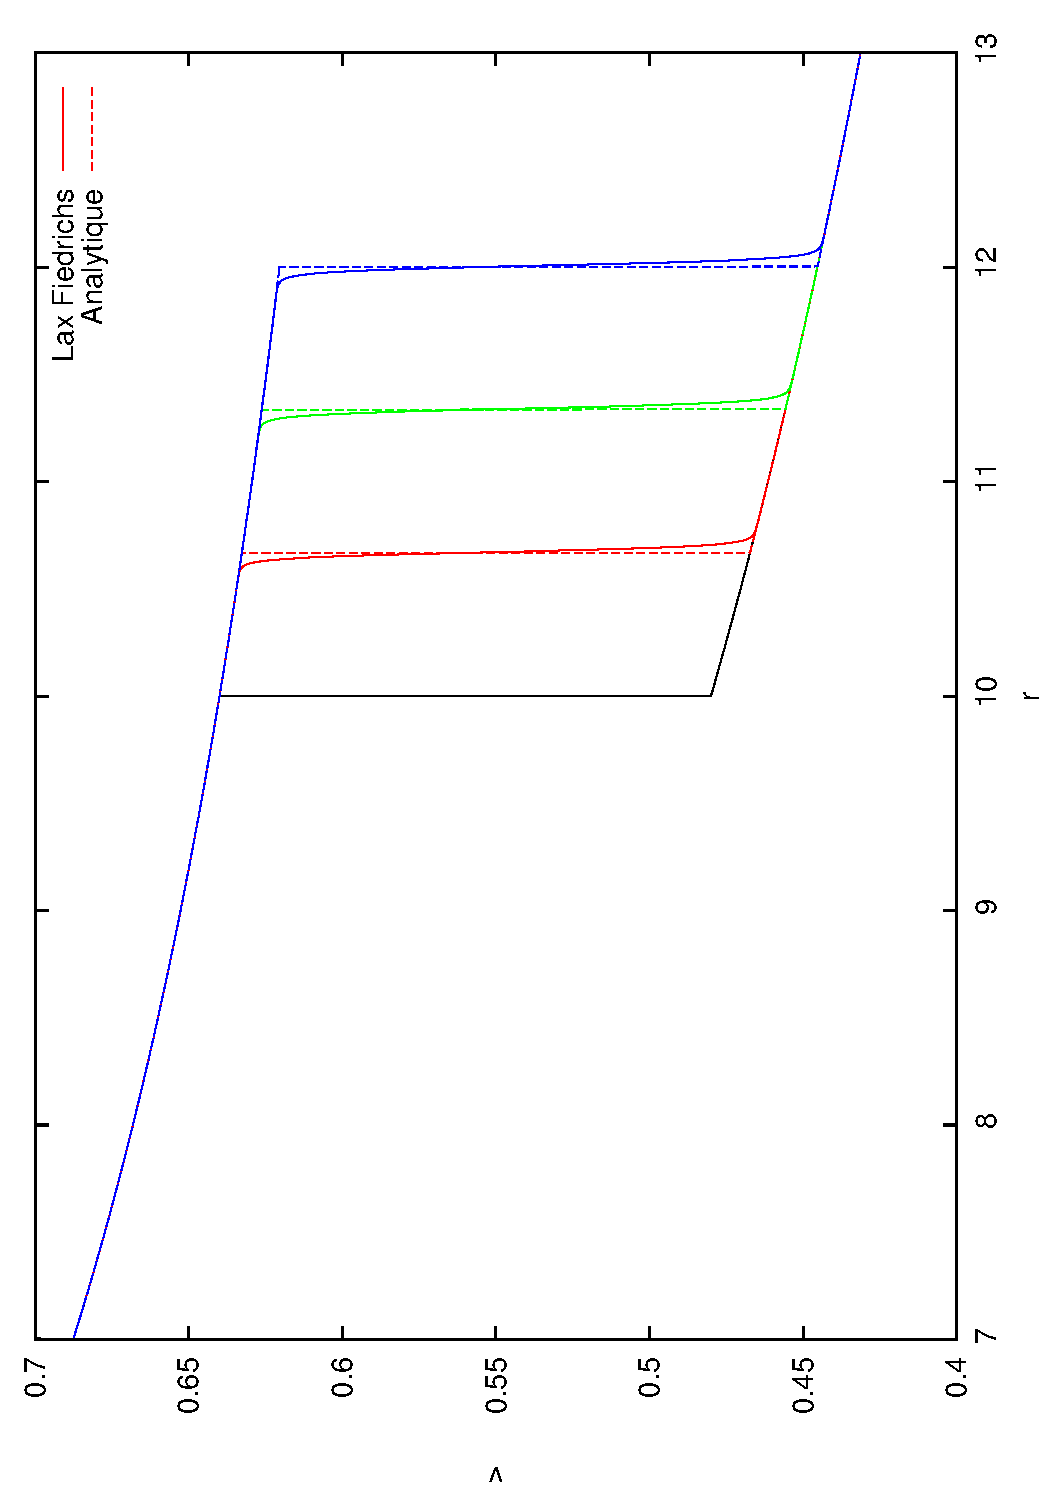
\includegraphics[scale=0.3, angle=-90]{figures/choc_lax.pdf}\label{choc_lax}}
\subfloat[Caractéristiques autour d'un choc]{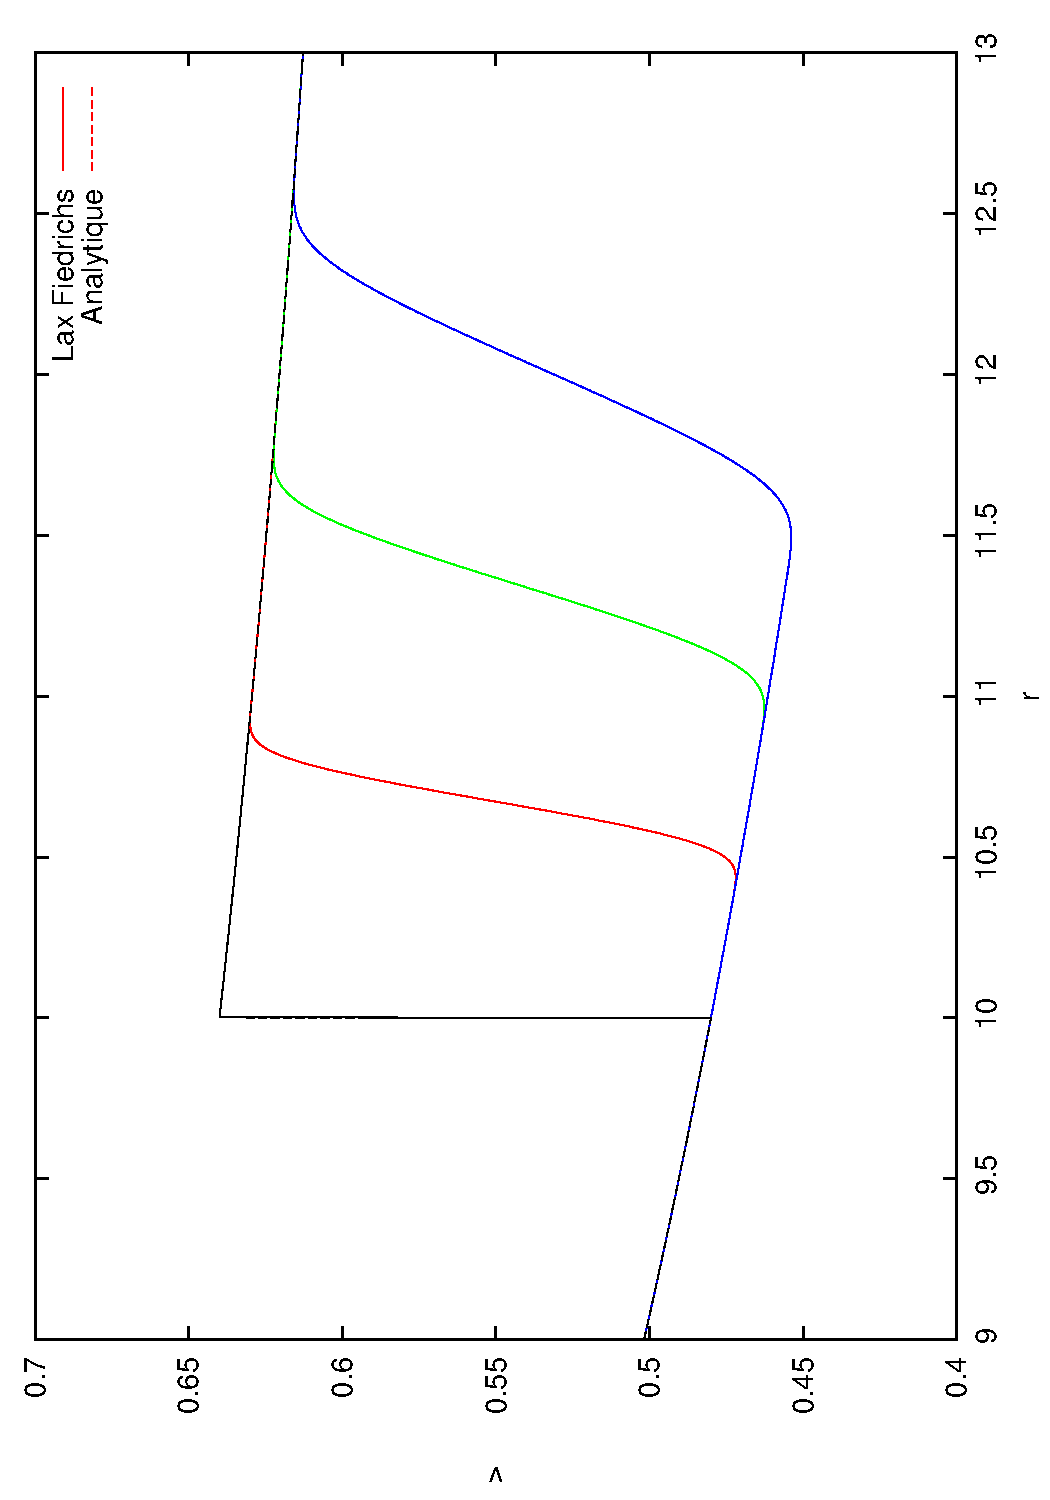
\includegraphics[scale=0.3, angle=-90]{figures/choc_lax_r.pdf}\label{rarefaction_lax}}
\caption{Nous avons tracé sur cette figure la solution du problème de Riemann obtenue par la méthode de Lax-Friedrichs, en la comparant avec la solution analytique. On y observe la présence de diffusion numérique au niveau des chocs et un accord parfait entre les deux solutions pour la raréfaction.}\label{figure_lax}
\end{figure}

\subsection{La méthode de Glimm}

Nous allons maintenant introduire la \textbf{méthode de Glimm} ou \textbf{méthode de choix aléatoire}, basée sur les travaux de J. Glimm \cite{glimm1965solutions}, qui a montré notamment la  convergence de la méthode, et de A. Chorin \cite{chorin1976random}, \cite{chorin1977random}. La version généralisée de cette méthode pour le modèle de Burgers relativiste est étudiée dans \cite{PLF-SX-one}. %Comme nous allons le voir, cette méthode s'appuie sur la résolution du problème de Riemann pour chaque itération en temps.%Elle a été introduite pour rendre compte de certain phénomènes de mécanique des fluide. %Cette méthode se base

\subsubsection{La version standard}

La méthode de Glimm consiste comme pour la méthode de Lax-Friedrichs à approximer la solution $v(x,t)$ de l'équation de Burgers aux points spatiaux $x_j = j\Delta x, \; j \in \mathbb{Z}$ pour les temps $t_n = n\Delta t,\; n\in \mathbb{N}$. %Cependant pour une raison que nous allons bientôt évoquer elle évalue aussi la solution aux points spatiaux $x_{j+1/2} = (j+1/2)\Delta x$ aux temps $t_{n+1/2} = (n+1/2)\Delta t$.
Nous l'appliquons par itérations successives pour faire progresser dans le temps la donnée initiale $u(x_j,0) = U_j^0,\; j\in \mathbb{Z}$. Pour passer du temps $t_n$ à $t_{n+1}$, on agit en deux étapes en commençant par faire évoluer la solution de $t_n$ à $t_{n+1/2}$ puis en la faisant évoluer de $t_{n+1/2}$ à $t_{n+1}$. Ces deux étapes étant similaires, nous ne présentons que le passage de $t_{n}$ à $t_{n+1/2}$.  
La méthode consiste premièrement à approximer la solution $v(x,t)$ au temps $t_n$ par une fonction constante par morceaux. Cette dernière est définie telle que pour chaque cellule $[x_{j-1/2},x_{j+1/2}]$, sa valeur soit donnée par $v(x_j, t_n)$.

On construit alors la solution analytique de l'équation de Burgers pour $t_n \leq t \leq t_{n+1/2}$, ayant pour donnée initiale la fonction constante par morceaux. Cela nous amène à devoir résoudre le problème de Riemann avec la condition initiale
\begin{equation}
	v(x,t_n) = \left\{
	\begin{array}{rl}
	U_j^n, &\quad \text{pour } x\leq (j+1/2)\Delta x,\\
	U_{j+1}^n,&\quad \text{pour } x>(j+1/2) \Delta x
	\end{array}
	\right.
\end{equation}
pour chaque $j$ et pour $t>t_n$.
En général, $U_j^n$ et $U_{j+1}^n$ sont différents et la condition initiale contient donc une discontinuité au point $x = (j+1/2) \Delta x$ qui va se propager en une onde de choc ou bien donner une onde de raréfaction comme nous l'avons vu en \ref{probleme_riemann_standard}. Si la condition CFL est vérifiée, deux chocs ne pourront pas interagir sur une même cellule nous permettant de recoller les solutions des problèmes de Riemann pour chaque $j$ et d'obtenir ainsi la solution de l'équation de Burgers au temps $t = t_{j+1/2}$.
Le c\oe ur de la méthode de Glimm consiste alors à tirer une variable aléatoire $\theta_{n+1/2}$ à valeurs dans $[-1,1]$ et d'assigner la valeur
\begin{equation}
	U^{n+1/2}_{j+1/2} = v\left(\left[j+\frac{1}{2} + \frac{1}{2}\theta_{n+1/2}\right]\Delta x,\left[n+1/2\right]\Delta t\right),
\end{equation}
à la solution approximée $U^{n+1/2}_{j+1/2}, \; j\in \mathbb{Z}$ dans la cellule $[x_j, x_{j+1}]$ au temps $t=t_{n+1/2}$.
On utilise ensuite la même procédure pour avancer du temps $t_{n+1/2}$ au temps $t_{n+1}$ et on répète ce processus en entier pour obtenir la solution approchée aux temps ultérieurs.

\subsubsection{La version généralisée}

Pour la méthode de Glimm généralisée, le principe est exactement le même que celui que l'on vient de voir pour le cas standard, à ceci près que nous n'approximons plus la donnée initiale par une fonction constantes par morceaux, mais \textbf{statique} par morceaux
\begin{equation}
	v(r,t_n) = \left\{
	\begin{array}{rl}
	v_L(r), &\quad \text{pour } r\leq (j+ 1/2) \Delta r,\\
	v_R(r),&\quad \text{pour } r> (j+ 1/2) \Delta r.
	\end{array}
	\right.
\end{equation}
où $v_L$ et $v_R$ sont les solutions statiques du modèle de Burgers relativiste \eqref{Burgers_relativiste_conservative}. Par conséquent, la méthode s'appuie à présent sur le \textbf{problème de Riemann généralisé} pour décrire l'évolution au cours du temps d'une discontinuité entre deux cellules voisines.% entre $t_n$ et $t_{n+1/2}$ ou $t_{n+1/2}$ à $t_{n+1}$

\subsubsection{Résultats numériques}

Comme pour la méthode de Lax-Friedrichs, nous terminons cette section en présentant les résultats obtenus  par la méthode de Glimm pour la résolution du modèle de Burgers généralisé. Le code source est présenté en annexe \ref{annexe}. Les valeurs de $v_L^0$ et $v_R^0$ sont toujours égales à $0.64$ et $0.48$ et la masse à $M=1$. Nous avons tracé la solution approchée et la solution analytique sur la figure \ref{fig:glimm_choc} pour un pas $\Delta t = 1\times 10^{-3}$ et un pas $\Delta r = 2\times 10^{-3}$.
La méthode n'introduit pas de diffusion numérique comme la méthode de Lax-Friedrichs mais diffère légèrement de la solution analytique. Ce dernier point est du au choix aléatoire que l'on fait pour attribuer sa valeur à la solution approchée au bout d'une (demi) itération en temps. Il faudrait alors encore diminuer le pas $\Delta t$ pour avoir un meilleur accord entre les deux solutions.

\begin{figure}\centering
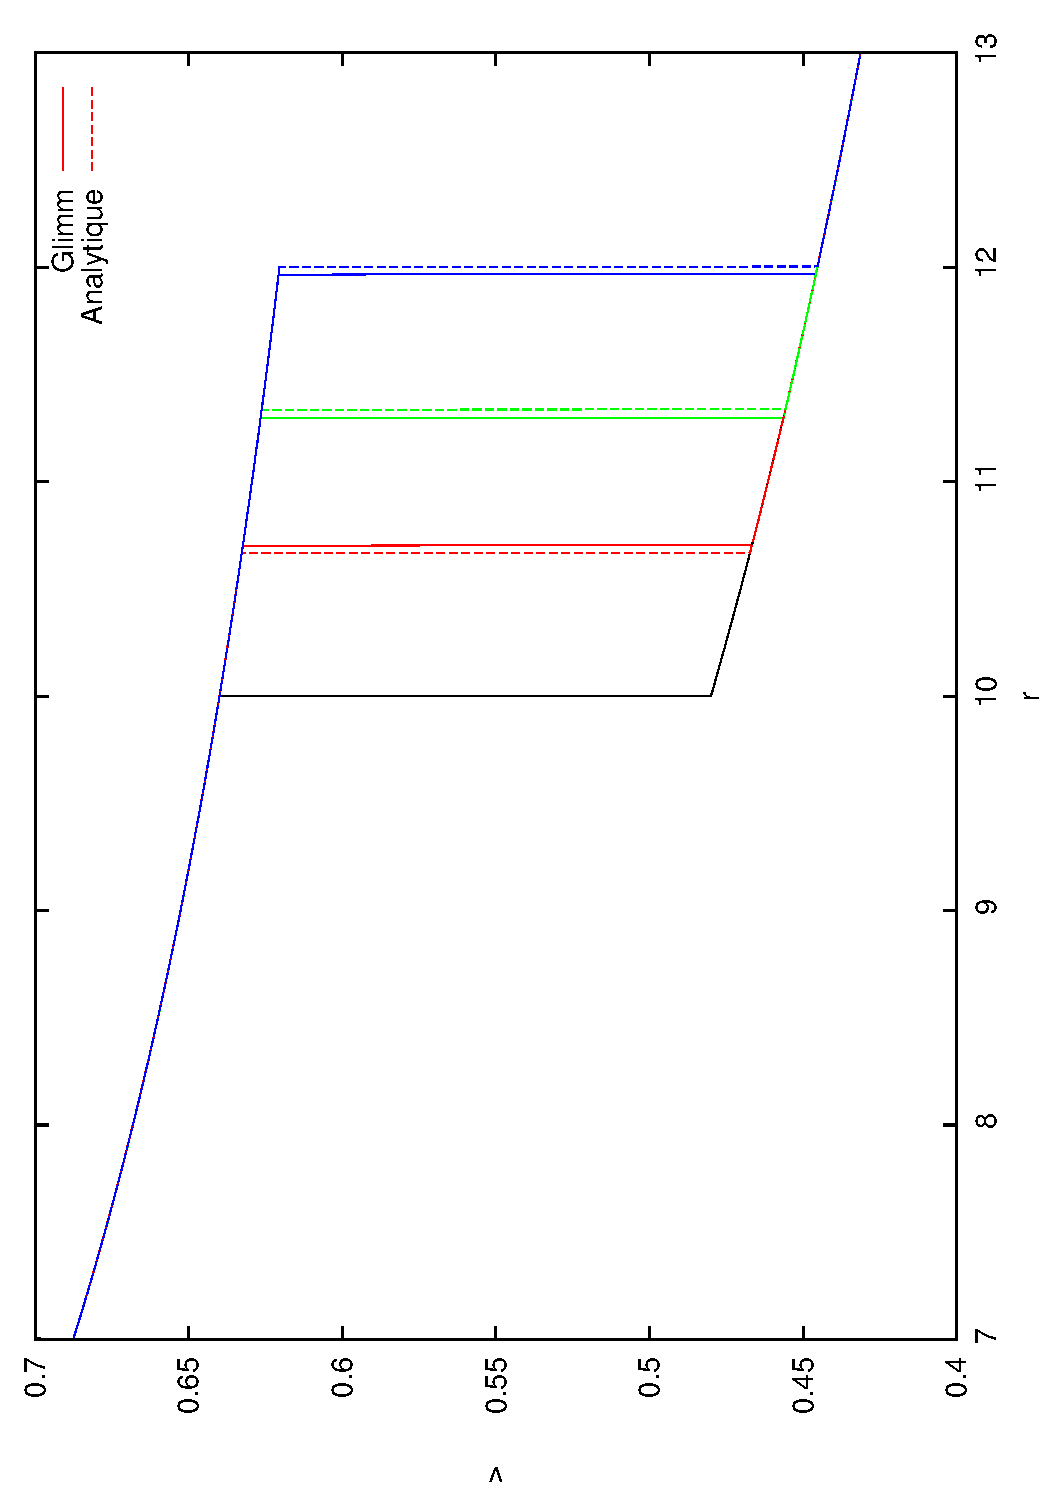
\includegraphics[scale=0.4, angle=-90]{figures/choc_glimm.pdf}
\caption{Nous avons tracé sur cette figure la solution du problème de Riemann obtenue par la méthode Glimm, en la comparant avec la solution analytique. La légère différence observée entre les deux est due au choix aléatoire que l'on fait pour approximer la solution à chaque itération en temps. En diminuant le pas $\Delta t$, on peut arriver à une meilleur accord.}
\label{fig:glimm_choc}
\end{figure}

\newpage
\section{Conclusion}

Après avoir introduit des concepts généraux sur les lois de conservation hyperboliques, nous avons dérivé le modèle de Burgers relativiste dans un espace de Schwarzschild. Nous avons alors cherché à élaborer une méthode de Lax-Friedrichs ainsi qu'une méthode de Glimm pour résoudre numériquement cette équation. La première comme dans le cas standard introduit de la diffusion numérique au niveau des chocs alors que la deuxième n'en introduit pas. La méthode de Lax-Friedrichs possède tout de même l'avantage de s'exprimer simplement au contraire de la méthode de Glimm qui a elle besoin de la solution du problème de Riemann généralisé pour pouvoir être appliquée. Le problème de Riemann généralisé que nous avons également introduit, voit les caractéristiques ainsi que les chocs de sa solution, qui étaient de simples droite dans le cas standard, devenir des courbes dont l'expression ne peut être obtenue qu'en résolvant une équation non-linéaire.
Chacune des deux méthodes qu'on a vu possède donc ses avantages et ses défauts.

Par manque de temps, nous n'avons malheureusement aborder que le cas du choc pour la méthode de Glimm et une suite à ce travail serait donc de s'intéresser au cas de la raréfaction. De plus, nous nous sommes placés uniquement dans le cas où $v_L^0$ et $v_R^0$ appartenaient au domaine des grandes vitesses. Cependant, nous avons vu que quand elles appartenaient au domaine des vitesses faibles, les solutions statiques n'étaient définies que localement. Ceci va donc amener de nouveaux problèmes dans l’implémentation de la méthode de Glimm si on se place dans ce régime. Enfin, tout ceci pourrait être un point de départ pour s'intéresser ensuite au cas vectoriel des équations d'Euler dans une espace courbe.

\newpage
\appendix

\section{Codes sources des différentes méthodes utilisées}\label{annexe}

Nous listons ici l'ensemble des codes sources que nous avons écrit en C99 pour la mise en \oe uvre des méthodes de Lax-Friedrichs et de Glimm. Nous listons premièrement les fichiers contenant les fonctions auxiliaires qui ne participent pas directement à la résolution des équations, avec certains des headers qui définisse les variables globales. Sont ensuite listés les fichiers pour la méthode de Lax-Friedrichs, puis ceux de la méthode de Glimm.

\subsection{Headers et fonctions auxiliaires}


\vspace*{0.3cm}
{\scalefont{.85}
\lstinputlisting{code_samples/real_precision.h}
}

\vspace*{0.5cm}
{\scalefont{.85}
\lstinputlisting{code_samples/io.c}
}

\vspace*{0.5cm}
{\scalefont{.85}
\lstinputlisting{code_samples/scan_real.c}
}

\vspace*{0.5cm}
{\scalefont{.85}
\lstinputlisting{code_samples/parametres.h}
}

\vspace*{0.5cm}
\newpage

\subsection{Lax-Friedrichs}

\vspace*{0.25cm}
{\scalefont{.85}
\lstinputlisting{code_samples/burgers.c}
}

\vspace*{0.25cm}
{\scalefont{.85}
\lstinputlisting{code_samples/methodes.c}
}
\newpage

\subsection{Glimm}

\vspace*{0.25cm}
{\scalefont{.85}
\lstinputlisting{code_samples/burgers_glimm.c}
}

\vspace*{0.25cm}
{\scalefont{.85}
\lstinputlisting{code_samples/methodes_glimm.c}
}

\newpage
\bibliographystyle{ieeetr}
\bibliography{bibliographie_stage_m2}

\end{document}
